\documentclass[a4paper,11pt]{article}
\pdfoutput=1

\usepackage{jheppub}

%\usepackage[T1]{fontenc} % if needed
\usepackage{amsmath,amssymb,graphicx}
\usepackage{subfigure}
\usepackage{multirow}
\usepackage{dcolumn}
\usepackage{color,url}
\usepackage{colordvi}
\usepackage{bm}
\usepackage{siunitx}
\usepackage{slashed}
\usepackage{natbib}
\usepackage{hyperref}
\usepackage{makecell}
\usepackage{pbox}
%\usepackage{fourier} 
\usepackage{array}
\newcommand{\bea}{\begin{eqnarray}}
\newcommand{\eea}{\end{eqnarray}}
\newcommand{\beq}{\begin{eqnarray}}
\newcommand{\eeq}{\end{eqnarray}} 
\newcommand{\CL}{{\cal L}}
\newcommand{\power}[2]{{#1}^{#2}}
\newcommand{\ud}{\mathrm{d}}
\newcommand{\arxiv}[1]{\href{http://arxiv.org/abs/#1}{\color{blue}{#1}}}

\newcommand{\mgamc}{Madgraph5\_aMC@NLO}
\newcommand{\whizard}{WHIZARD}

\newcommand{\xznote}[1]{\textbf{[X.Z.:}\textit{\textcolor{blue}{\Large #1}}\textbf{]}}

\newcommand{\bra}[1]{\langle#1|}
\newcommand{\ket}[1]{|#1\rangle}

\newcommand{\gwa}[1]{g_{W,a#1}}
\newcommand{\gwb}[1]{g_{W,b#1}}
\newcommand{\gwc}[1]{g_{W,c#1}}
\newcommand{\gza}[1]{g_{Z,a#1}}
\newcommand{\gzb}[1]{g_{Z,b#1}}
\newcommand{\gaa}[1]{g_{A,a#1}}
\newcommand{\gab}[1]{g_{A,b#1}}
\newcommand{\gzc}[1]{g_{Z,c#1}}
\newcommand{\gva}[1]{g_{V,a#1}}
\newcommand{\gvb}[1]{g_{V,b#1}}
\newcommand{\gxa}[1]{g_{X,a#1}}
\newcommand{\gxb}[1]{g_{X,b#1}}

\def\missE{\slashed E} % missing E

\title{\boldmath Measuring B anomalies by $\mu^+\mu^-\to t\bar{c}$ at future lepton colliders}

%\author[a]{Wolfgang Kilian}
\author[a]{Sichun Sun}
\author[b,c]{Qi-Shu Yan}
\author[d]{Xiaoran Zhao}
\author[c,e]{Zhijie Zhao}

%\affiliation[a]{Department of Physics, University of Siegen, 57072 Siegen, Germany}
\affiliation[a]{Department of Physics, National Taiwan University, Taipei, Taiwan}
\affiliation[b]{School of Physics Sciences, University of Chinese Academy of Sciences, Beijing 100039, China}
\affiliation[c]{Center for Future High Energy Physics, Institute of High Energy Physics, Chinese Academy of Sciences, Beijing 100039, China}
\affiliation[d]{Dipartimento di Matematica e Fisica, Universit{\`a} di Roma Tre and \\
INFN, sezione di Roma Tre, I-00146 Rome, Italy}
\affiliation[e]{DESY, Notkestr. 85, 22607 Hamburg, Germany}


%\emailAdd{kilian@physik.uni-siegen.de}
\emailAdd{sichunssun@gmail.com}
\emailAdd{yanqishu@ucas.ac.cn}
\emailAdd{xiaoran.zhao@uniroma3.it}
\emailAdd{zhijie.zhao@desy.de}

\preprint{SI-HEP-2018-27,CP3-18-55,MCnet-18-21}


\abstract{
Being motivated from B anomalies, we study the match procedure of operators in the effective Hamiltonian in mass eigenstates and operators in the weak eigenstates. It is noticed that there are more operators in the SMEFT which can not simply being fixed from the low energy data from the B anomalies. We demonstrate this matching procedure with some new physics models, like $Z^\prime$ model and leptoquark models, and then consider how to probe these operators of SMEFT by using the process $\mu^+\mu^-\to tc$ at future muon colliders, which can provide complementary information on the underlying models which lead to B anomalies. We have performed a simple Monte Carlo simulation to show how to separate the signal events from the SM background events, and have estimated the sensitivity to the Wilson coefficients for different models.
}

\begin{document}
\maketitle
\flushbottom


\section{Introduction}
Searching for new physics is the prime target of both high energy frontier and high precision frontier.
In the rare decays of B mesons, there exist long standing discrepances between the Standard Model predictions and experimental measurements, with a hint of non-lepton flavor universality(LFU), especially in the muon related final states. These B-anomalies are observed in a $B \rightarrow K \mu^+ \mu^-$,  $B_s \rightarrow \phi  \mu ^+ \mu^-, B_s \rightarrow  \mu ^+ \mu^-$ and angular distribution of  $B \rightarrow K^* \mu ^+ \mu^-$\cite{LHCb:2021awg,LHCb:2021vsc,LHCb:2017rmj,ATLAS:2018cur,CMS:2019bbr}. For the LFU violation, it has been observed by LHCb\cite{LHCb:2021trn,LHCb:2019hip,LHCb:2017avl,LHCb:2015svh,LHCb:2020lmf,LHCb:2020gog} in the ratio 

\begin{eqnarray}
R_K = \frac{BR(B \rightarrow K \mu^+ \mu^-)}{BR(B \rightarrow K e^+ e^-)}, R_{K^*} = \frac{BR(B \rightarrow K^* \mu^+ \mu^-)}{BR(B \rightarrow K^* e^+ e^-)}
\end{eqnarray}

Altough large hadronic uncertainties can enter in some of these absolute branching fractions and angular observables for the Standard model predictions, $R_K, R_{K^*}, B_s \rightarrow  \mu ^+ \mu^- $ are considered relatively theoretically clean. The deviation in those measurements might lead to indirect evidence for new physics \cite{Hiller:2014ula, Altmannshofer:2017fio, Altmannshofer:2014rta,Geng:2017svp,Ciuchini:2019usw,Datta:2019zca,Aebischer:2019mlg,Ciuchini:2020gvn,Jager:2017gal}. While those measurement provides derivation from SM prediction,
the exact mechanics behind those anomaly are still unknown,
and low-energy measurement couldn't fully reveal the nature behind that.

On the other hand, by scattering high energy particles,
collider experiments provide unique opportunities to access underlying UV theories.
Among various current and future colliders\cite{Shiltsev:2019rfl},
a multi-TeV muon collider\cite{Aime:2022flm,MuonCollider:2022xlm} is ideal for such studies.
Being fundamental particles, the entire energy of incoming muons are available to produce short-distance scattering rather than being spread among partons of hadrons,
and thus a 14 TeV muon collider could be as effective as a 100 TeV proton-proton collider\cite{Delahaye:2019omf}.
Such high energy reach strongly benefits to searching new heavy particles, such as minimal dark matter models\cite{Han:2020uak,Bottaro:2021snn},
as well as indirect measurement at high energies\cite{Buttazzo:2020uzc}.
Moreover, vector boson fusion processes are found to be important at muon colliders\cite{Costantini:2020stv},
and enable access to difficult parameters such as the Higgs quartic self-coupling\cite{Chiesa:2020awd}.
More importantly, muon colliders have a special feature: the initial states are muons, directly related to those low-energy anomalies. The muon $g-2$ anomaly could be probed directly at muon colliders\cite{Buttazzo:2020ibd},
In the context of muon $g-2$ anomaly, studies have been performed on testing it under the SMEFT formalism\cite{Buttazzo:2020ibd}, and model-exhaustive analysis\cite{Buttazzo:2020ibd,Capdevilla:2020qel,Capdevilla:2021rwo,Capdevilla:2021kcf}.
%The future collider proposals include the linear or circular case $e^+e^-$ colliders\cite{} and circular pp coliders \cite{}, and especially relevant here: high-energy muon colliders \cite{}.  Muon colliders can reach high energies with large mass suppression of synchroton radiation comparing to $e^+e^-$ colliders and higher precision with cleaner final states comparing to pp colliders. Although the short life time of muon causes some technical challenges, there are a series of recent progresses\cite{}.

 The multi-TeV reach and better precision advantages of muon colliders, makes a perfect place to probe muon related B anomalies in low energy. There are already proposals studying $\mu^+\mu^-\to b\bar{s}$ or $\bar{b}s$ at multi TeV scale to discuss the impact of low energy B-anomalies impact \cite{Altmannshofer:2022xri,Huang:2021nkl}. At the current stage, B-anomalies can be nicely accommodated by effective four-fermion operators at B-physics scale ($\mu= 4.8$ GeV):
 \begin{eqnarray}
   O_9 &=& (\bar{s}\gamma_\mu P_L b)(\bar{\ell}\gamma^{\mu}\ell),  \\
   O_{10} &=& (\bar{s}\gamma_\mu P_L b)(\bar{\ell}\gamma^{\mu}\gamma_5\ell),
\end{eqnarray}
For the new physics effects described by operators $O_9$ and $O_{10}$, when we go above the weak scale ($\mu=M_Z$ for instance), the Wilson coefficients of such two operators depend on the specific models (e.g. leptoquark, scalars,$Z'$,etc). 

In this work, we adopt the same assumption that the new physics scale is around $\mu=35$ TeV and it is challenging to discover the new physics signature at the LHC. We also assume that these new physics above the weak scale ($\mu=M_Z$) can be described by the framework of the standard model effective field theory (SMEFT). Under appropriate assumptions, it is noteworthy that there are at least one more operator is needed in order to match the SMEFT to low energy operators $O_9$ and $O_{10}$. These three operators in the SMEFT are given in Eqs. (2.12-2.14). Different new physics models can lead to different matching conditions across the weak scale.

Different from the proposal presented in \cite{Altmannshofer:2022xri}, where the polarization of muon beams and charge tagging of jets in the final state are assumed, in this work, in order to reveal the nature of new physics which leads to the B anomalies, we propose to measure the process $\mu^+\mu^-\to tc$ (here $tc$ denotes both $t \bar{c}$ and $\bar{t} c$), which can provide complementary information to the processes $\mu^+\mu^-\to b \bar{s}$ ($\bar{b} s$). The four fermion operators for $\mu^+\mu^-\to tc$ naturally arise from the operator matching conditions from low energy effective field theory to the SMEFT, since left-handed top and charm quarks form an electroweak SU(2) doublets as the partners of the left-handed bottom and strange quarks in SMEFT operators. We can also observe that the process $\mu^+\mu^-\to tc$ can help to distinguish different new physics models, which can yield different operator matching conditions. We will consider a $Z^\prime$ model and a few leptoquark models. 

The leptoquark particles are predicted in the grand unification models and they could either be scalar or vector bosons. Usually, these particles should be superheavy (say $10^13$ GeV), as required by the experimental data of proton decays. Very light leptoquarks (say 1 TeV or a few 10 TeV) can be consistent with experimental data if their couplings to the first generation of matter fields are weak. Light leptoquarks are also predicted in the Pati-Salam model, where lepton numbers are treated as the forth color quantum number. These light leptoquarks could be even accessible at the LHC and future collider projects. Recently, leptoquarks have attracted much attentions in order to interpret the B anomalies. A comprehensive on the phenomenology of leptoquark can be found in \cite{Dorsner:2016wpm}.

\textcolor{blue}{Our main findings} Our new findings include: 1)  The dominant background events of the SM for the process $\mu^+\mu^-\to tc$ are different from those of the process $\mu^+\mu^-\to bs$. Due to the highly boosted top quark in the final states, jet substructure analysis can be crucial to distinguish signal and background events. 2) In the case that there is no new resonance which will be found the TeV muon colliders, measurement of the process $\mu^+\mu^-\to tc$, can provide crucial information on the potential nature of the new physics which leads to the low energy B anomalies. 3) The weak final state radiation might become important for such a measurement.

This paper is organized as given below. In section II, we demonstrate the relations between the Wilsonian coefficients of the effective Hamiltonian and those of the SMEFT. In section III, we present the values of Wilsonian coefficients of the SMEFT derived from different new physics models. These new physics models can accommodate the data of B anomalies. In section IV, we perform a Monte Carlo simulation to explore the sensitivity of future muon colliders to these new physics scenarios. We end this work with a few discussion and conclusion. In Appendix, we present the renormalization group equations of Wilsonian coefficients in the SMEFT and effective Hamiltonian, respectively. 


%\section{Motivations for studying B-anomalies in $\mu^+\mu^-\to tc$}
\section{Matching and RGE of different operator bases}
\label{Sec:EFT}

 Interestingly, these anomalies can be simultaneously explained in form of a model-independent way with the effective four-fermion operators. 
In many researches of B-physics,  new physics effects strongly prefer an effective Hamiltonian with $O_9 $ and $O_{10}$ with Wilson coefficients of dimension 6 interactions at the renormalization scale $\mu =4.8$ GeV ,
\begin{eqnarray}
  \mathcal{H}_{eff} &=& \mathcal{H}^{SM}_{eff}-\mathcal{N}\sum_{\ell=e,\mu}\sum_{i=9,10}\left(c_iO^{bs\ell\ell}_i+c^\prime_i O^{\prime bs\ell\ell}_i\right) + h.c., 
\end{eqnarray} 
where the normalization factor $\mathcal{N}$ is 
\begin{eqnarray}
  \mathcal{N} &=& \frac{4G_F}{\sqrt{2}}V_{tb}V^*_{ts}\frac{e^2}{16\pi^2}. 
\end{eqnarray}
The operators $O_9$ and $O_{10}$ are 
\begin{eqnarray}
   O^{bs\ell\ell}_9 &=& (\bar{s}\gamma_\mu P_L b)(\bar{\ell}\gamma^{\mu}\ell),  \\
   O^{bs\ell\ell}_{10} &=& (\bar{s}\gamma_\mu P_L b)(\bar{\ell}\gamma^{\mu}\gamma_5\ell),
\end{eqnarray}
where $P_L=(1-\gamma_5)/2$ is the left-handed projection operator. 
For $O^\prime_i$, $P_L$ is replaced by right-handed projection operator $P_R=(1+\gamma_5)/2$.

For the purpose of this paper, to study B-anomalies related operator $O_9$ and $O_{10}$ defined in the low energy B physics scale in higher colliding energy scale, we need to treat the running and matching of the operators carefully. 
Especially the subtleties arise when the energy running across the weak scale. Our study finds that in the energy scale above the weak scale, the impact of $O_9$ and $O_{10}$ operators needs to be reparametrized by three different operators, rather than two, in so-called Warsaw basis, known as the Standard model effective theory (SMEFT). Here we introduce different basises and coefficient matching as below. 

 At the scale below the weak scale, potential new physics effects are described by a low energy effective field theory (LEFT).  
The LEFT Lagrangian with dimension 6 operators can be written as 
\begin{eqnarray}
  \mathcal{L}_{LEFT} &=& \mathcal{L}_{QCD+QED}+ \frac{1}{v^2}\sum_{i}L_iQ_i,  \nonumber 
\end{eqnarray} 
where $L_i$ are the Wilson Coefficients of LEFT, and $v=246$ GeV is the vacuum expectation value. 

In this paper, we use the convention of Ref.~\cite{Jenkins:2017jig}. 
The most relevant operators are 
\begin{eqnarray}
  Q^{V,LL}_{ed}(p,r,s,t) &=& (\bar{e}_{Lp}\gamma^\mu e_{Lr})(\bar{d}_{Ls}\gamma_\mu d_{Lt}),  \label{QVLLed} \\
  Q^{V,LR}_{de}(p,r,s,t) &=& (\bar{d}_{Lp}\gamma^\mu d_{Lr})(\bar{e}_{Rs}\gamma_\mu e_{Rt}),  \label{QVLRde}
\end{eqnarray}
where $p,r,s,t$ are generation indices of quark or lepton. 
Since the EW symmetry is broken, here $e$ and $d$ are the lepton field and down-type quark field. 
$L$ and $R$ are the chiral indices of fermions. 



One can derive the relations between $Q_i$ and $O_i$ easily:
\begin{eqnarray}
  Q^{V,LL}_{ed} &=& \frac{1}{2}\left(O_9-O_{10}\right),  \\
  Q^{V,LR}_{de} &=& \frac{1}{2}\left(O_9+O_{10}\right).   
\end{eqnarray}
So we have 
\begin{eqnarray}
  L^{V,LL}_{ed} &=& \frac{\mathcal{N}v^2}{2}(c_9-c_{10}),  \\
  L^{V,LR}_{de} &=& \frac{\mathcal{N}v^2}{2}(c_9+c_{10}). 
\end{eqnarray}
The constraints of $c_9$ and $c_{10}$ can be found in Ref.~\cite{Altmannshofer:2021qrr}.

Assuming the new physics appears at a scale above the weak scale $\Lambda$, 
the SMEFT Lagrangian with dimension 6 operators ($\mathcal{O}_i$) is defined as
\begin{eqnarray}
  \mathcal{L}_{SMEFT} &=& \mathcal{L}_{SM} + \frac{1}{\Lambda^2}\sum_{i}C_i\mathcal{O}_i,  
\end{eqnarray}
where $C_i$ are called Wilson Coefficients.

A complete set of non-redundant dimension 6 operators has been derive in Ref.~\cite{Grzadkowski:2010es}, so-called Warsaw basis. 
The most relevant operators in this paper are
\begin{eqnarray}
   \mathcal{O}^{(1)}_{lq}(p,r,s,t) &=& (\bar{l}_p\gamma^\mu l_r)(\bar{q}_s\gamma_\mu q_{t}),  \label{O1lq} \\
   \mathcal{O}^{(3)}_{lq}(p,r,s,t) &=& (\bar{l}_p\gamma^\mu\tau^I l_r)(\bar{q}_s\gamma_\mu\tau^I q_{t}),  \label{O3lq} \\
   \mathcal{O}_{qe}(p,r,s,t) &=& (\bar{q}_p\gamma^\mu q_r)(\bar{e}_s\gamma_\mu e_t), \label{Oqe}
\end{eqnarray}
where $q$, $l$, $e$ are the left-handed quark doublet, left-handed lepton doublet, and right-handed lepton singlet, respectively. 
$p,r,s,t$ are generation indices of quark or lepton.

When the electroweak symmetry breaking occurs, the SM heavy particles (top, Higgs,  $W^\pm$,  $Z$) are integrated out, and the SMEFT should be matched to LEFT. 
The full matching conditions at tree level have been derived by Ref.~\cite{Jenkins:2017jig}.
In this paper, we only consider the operators with flavour indices $(p,r,s,t)=(2,2,2,3)$ or $(p,r,s,t)=(2,3,2,2)$, so the matching conditions are simplified to 
\begin{eqnarray}
    L^{V,LL}_{ed}(2,2,2,3) &=& \frac{v^2}{\Lambda^2}\left[C^{(1)}_{lq}(2,2,2,3)+C^{(3)}_{lq}(2,2,2,3)\right],  \label{match:VLLed}\\
    L^{V,LR}_{de}(2,3,2,2)&=& \frac{v^2}{\Lambda^2}C_{qe}(2,3,2,2). \label{match:VLRde}
\end{eqnarray}
% \bigskip
The related renormalization group equations for the SMEFT and LEFT can be found in the Appendix \ref{smeftrge} and Appendix \ref{leftrge}, respectively.

\begin{center}
\begin{table}
  \begin{center}
  \begin{tabular}{c|cccc}
  \hline
  &      $c_9=-0.73, c_{10}=0$    &     $c_9=0, c_{10}=0.54$      &       $c_9=c_{10}=0.05$     &       $c_9=-c_{10}=-0.39$       \\
  \hline
                   $L^{V,LL}_{ed}(m_B)$ &   $-1.727\times 10^{-5}$   &   $-1.278\times 10^{-5}$   &  $0$    &    $-1.845\times 10^{-5}$    \\
                   $L^{V,LL}_{ed}(m_Z)$  &   $-1.748\times 10^{-5}$  &   $-1.287\times 10^{-5}$   &  $5.651\times 10^{-9}$  &  $-1.863\times 10^{-5}$  \\
                   $(C^{(1)}_{lq}+C^{(3)}_{lq})(m_Z)$  &   $-0.029$  &    $-0.021$   &   $9.337\times 10^{-6}$  &  $-0.031$  \\
                   $(C^{(1)}_{lq}+C^{(3)}_{lq})(\Lambda)$  &  $-0.030$   &  $-0.023$  &  $2.053\times 10^{-5}$  &  $-0.032$ \\ 
  \hline
  $L^{V,LR}_{de}(m_B)$ &  $-1.727\times 10^{-5}$  & $1.278\times 10^{-5}$ & $2.366\times 10^{-6}$ & $0$ \\ 
  $L^{V,LR}_{de}(m_Z)$ & $-1.723\times 10^{-5}$  & $1.268\times 10^{-5}$ &  $2.355\times 10^{-6}$ & $-4.408\times 10^{-8}$   \\
  $C_{qe}(m_Z)$  &   $-0.028$   &  $2.096\times 10^{-2}$  & $3.891\times 10^{-3}$ &  $-7.283\times 10^{-5}$ \\
  $C_{qe}(\Lambda)$  &  $-0.029$   &  $2.142\times 10^{-3}$  &   $3.993\times 10^{-3}$   &  $-2.019\times 10^{-4}$  \\
  \hline
  \end{tabular}
  \end{center}
  \caption{The coefficients $L^{V,LL}_{ed}$, $L^{V,LR}_{de}$, $C^{(1)}_{lq}+C^{(3)}_{lq}$ and $C_{qe}$ at scale $m_B=5$ GeV, $m_Z=91.1876$ GeV and $\Lambda=10$ TeV are listed, with difference input of $c_9$ and $c_{10}$. Here, we assume $C^{(1)}_{lq}=3C^{(3)}_{lq}=\frac{3}{4}L^{V,LL}_{ed}\times \Lambda^2/v^2$. \label{table:LVLLed}}
\end{table}
\end{center}

\section{The Matching Conditions of New Physics}


At muon colliders, the operators we input are actually Eq. (\ref{Oqe}).
 In massless limit,\footnote{For simplicity, in this section we work under massless limit. Nevertheless, for the numerical results discussed in later sections, full mass dependence are included} the differential cross section for $\mu^+\mu^-\to tc$ and  $\mu^+\mu^-\to bs$ are:
 \begin{align}
     \frac{\ud\sigma(\mu^+\mu^-\to X)}{\ud\cos\theta}=\frac{3s}{256\pi}|C_{LL}^{X}|^2(1+\cos\theta)^2
 \end{align}
 where
 \begin{align}
 C_{LL}^{bs}=C_{lq}^{(1)}+C_{lq}^{(3)},C_{LL}^{tc}=C_{lq}^{(1)}-C_{lq}^{(3)}
 \end{align}

Integrating over $\cos\theta$, we can obtain the inclusive cross section as:
\begin{align}
    \sigma(\mu^+\mu^-\to X)=\frac{1}{32\pi}s|C_{LL}^{X}|^2
\end{align}

In a general new physical model,
both $C_{lq}^{(1)}$ and $C_{lq}^{(3)}$ can be non-zero,
and thus both processes $\mu^+\mu^-\to tc$ and $\mu^+\mu^-\to bs$ receives new physical contribution,
and can be measured in future muon colliders.
We note that for $\mu^+\mu^-\to bs$, the corresponding Wilson coefficients $C_{LL}^{bs}$ is directly in charge of $b\to s\mu^+\mu^-$ transition in $B$-physics,
and hence constrained by those measurements.
On the other hand, $C_{LL}^{tc}$ is unconstrained.
As a general argument, the underlying new physical which induce $C_{LL}^{bs}$ or equivalently $C_{lq}^{(1)},C_{lq}^{(3)}$,
would induce also $C_{LL}^{tc}$ with size at similar order.

Therefore, we expect that the cross section of $\mu^+\mu^-\to tc$ is comparable to $\mu^+\mu^-\to bs$,
and as we will show in Section \ref{Sec:result}, due to the presence of top quark in the final state of $\mu^+\mu^-\to tc$,
it is easier to measure than $\mu^+\mu^-\to bs$.
To be more specific, below we discuss four types of new physics models labelled as Model I-IV, 
where the relations between $C_{LL}^{tc}$ and $C_{LL}^{bs}$ are given,
and later in Section \ref{Sec:result} we will show how to distinguish them by measuring both $\mu^+\mu^-\to tc$ and $\mu^+\mu^-\to bs$.

\begin{enumerate}
    \item[Model I]   A $Z^{\prime}$ mdoel with flavor symmetry $U(1)_{L_{\mu}-L_{\tau}}$.
        In this model, the $L_{\mu}-L_{\tau}$ is promoted into a $U(1)$ gauge symmetry,
        which is mediated by a massive gauge boson $Z^{\prime}$.
    Originally it was proposed for muon $g-2$ anomaly \cite{Baek:2001kca} and neutrino mixing \cite{Ma:2001md}.
    Later it is realised that its coupling to quarks can be described by high dimensional operators, which can be generated through new heavy quarks \cite{Fox:2011qd}.
    Such interaction can induce flavor violation \cite{Altmannshofer:2014cfa}, to explain B anomaly.
    Since the effective interaction between $bs\mu\mu$($tc\mu\mu$) is mediated by an $s$-channel $Z^{\prime}$, which is an electroweak singlet,
    clearly $C_{lq}^{(3)}=0,C_{LL}^{bs}=C_{LL}^{tc}=C_{lq}^{(1)}$.
    Consequently, we have $\sigma(tc)\sim\sigma(bs)$.

    \item[Model II] A scalar triplet leptoquark $S_3$ model.
        In this model, the new physics are mediated by a heavy scalar leptoquark, which belongs to $SU(2)_L$ triplet.
        The corresponding Lagrangian can be written as \cite{Dorsner:2016wpm}
        \begin{align}
            \mathcal{L}_{NP}=\sum_{i,j}\lambda_{ij}\bar{Q}_i^c(i\tau^2)\tau^{I}L_jS_3^{I}+\textrm{h.c.}
        \end{align}
        In this model, both $C_{lq}^{(1)}$ and $C_{lq}^{(3)}$ can be generated at tree-level, which is given by \cite{Gherardi:2020det}
        \begin{align}
            [C_{lq}^{(1)}]_{prst}=&3\frac{\lambda_{sp}^{*}\lambda_{tr}}{4M^2}\\
            [C_{lq}^{(3)}]_{prst}=&\frac{\lambda_{sp}^{*}\lambda_{tr}}{4M^2}.
        \end{align}
        where $M$ is the mass of the leptoquark $S_3$.
        Therefore, we have $C_{LL}^{bs}=2C_{LL}^{tc}$,
        and $\sigma(tc)=\frac{1}{4}\sigma(bs)$

    \item[Model III] A scalar singlet leptoquark $S_1$ model.
        In this model, new physics are mediated by a heavy scalar leptoquark, which belongs to $SU(2)_{L}$ singlet.
        There are three possible hypercharge assignments,
        and we consider the case $Y=\frac{1}{3}$ here.
        The corresponding Lagrangian is
        \begin{align}
            \mathcal{L}_{NP}=\sum_{i,j}\lambda_{ij}\bar{Q}^c_i(i\tau_2)L_jS_1+\textrm{h.c.}
        \end{align}
        At tree-level, the relevant Wilson coefficients are
        \begin{align}
            [C_{lq}^{(1),\textrm{tree}}]_{prst}=\frac{\lambda_{sp}^{L*}\lambda_{tr}^{L}}{4M^2}\\
            [C_{lq}^{(3),\textrm{tree}}]_{prst}=-\frac{\lambda_{sp}^{L*}\lambda_{tr}^{L}}{4M^2}
        \end{align}
        Interestingly, we can see that at tree-level $C_{LL}^{bs}=0$.
        The leading contribution to $C_{LL}^{bs}$ starts from one-loop level \cite{Bauer:2015knc}.
        Consequently, we expect that $C_{LL}^{bs}\ll C_{LL}^{tc}$,
        and hence $\sigma(tc)\gg C_{LL}^{bs}$.
        For the experiment bounds($C_9=-1$ benchmark point), we get
        \begin{align}
            \sum_{i}|\lambda_{u_i\mu}|^2\mathrm{Re}\frac{(\lambda\lambda^{\dag})_{bs}}{V_{tb}V_{ts}^{*}}-1.74|\lambda_{t\mu}|^2\sim 12.5\hat{M}^2
        \end{align}
        where $\hat{M}$ is the mass of the leptoquark in terms of unit TeV,
        and from $B_s-\bar{B}_s$ mixing we have
        \begin{align}
            \frac{(\lambda\lambda^{\dag})_{bs}}{V_{tb}V_{ts}^{*}}\sim(1.87+0.45i)\hat{M}
        \end{align}
        For perturbativity, we have $|\lambda_{u_i\mu}|^2<4\pi$, which yield
        \begin{align}
            M\lesssim 1.9\si{TeV}
        \end{align}
        Consequently, we expect that at the energy range of future muon colliders, it can be produced on-shell, and be observed directly.
\item[Model IV] A $U_1$ vector leptoquark model. Originally proposed in \cite{Barbieri:2015yvd},
see also \cite{Buttazzo:2017ixm}.
        The Lagrangian is given by
        \begin{align}
        \mathcal{L}_{NP}=-\frac{1}{2}U_{1,\mu\nu}^{\dag}U^{1,\mu\nu}+M_U^2U_{1,\mu}^{\dag}U_1^{\mu}+g_UU_{1,\mu}\lambda_{ij}\bar{Q}_{i}\gamma^{\mu}L_{j}+\textrm{h.c.}
        \end{align}
        The relevant Wilson coefficients are
        \begin{align}
            [C_{lq}^{(1),\textrm{tree}}]_{prst}=g_U^2\frac{\lambda_{sp}^{L*}\lambda_{tr}^{L}}{2M^2}\\
            [C_{lq}^{(3),\textrm{tree}}]_{prst}=g_U^2\frac{\lambda_{sp}^{L*}\lambda_{tr}^{L}}{2M^2}
        \end{align}
        Clearly, in this case we have $C_{LL}^{tc}\sim0,C_{LL}^{bs}\gg C_{LL}^{tc}$.
\end{enumerate}

\section{Signatute of $\mu^+\mu^-\to t\bar{c}$ at future muon colliders }
\label{Sec:result}

To study the $\mu^+\mu^-\to t\bar{c}$ process at future muon collider, 
we generate a UFO model with relevant operators by Feynrules~\cite{Alloul:2013bka}, 
and import it to \mgamc \cite{Alwall:2014hca}. 
We calculate the cross sections of signals and backgrounds from $E_{cm}=1$ TeV to $30$ TeV.  
The energy dependencies of the cross sections are shown in the Fig.~\ref{ecm}. 
The main background processes include $j j$, $W^+ W^-$, $t \bar{t}$, and $Zh$. The process $jj W^\pm$ is also included, which describes the weak final state radiation. These processes are from S-channel and decrease with the increase of the collision energy.

The cross section of main signal process $\mu^+ \mu^- \to t \bar{c} (\bar{t} c)$ derived from the 4-fermion interactions are proportional to collision $s^2$, and it increases with the increase of the collision energy, as shown in Figure 1. 
The largest signal is the case that only $c_{9}$ is switched on, and it can reach $\mathcal{O}(1)$ fb at the $30$ TeV. 

Near the threshold, cross section of all background processes are huge when compared with the signal process. With the increase of collision energy, the signal cross section can even be larger than those of background processes if the collision energy is large enough (say $\sqrt{s}=30$ TeV) for some new physics models. 
Nonetheless, when $\sqrt{s}=10$ TeV, it might be still challenging to discover the signal events since the cross section of background processes are several orders larger than that of the signals processes.

\begin{figure}
  \centering
  \subfigure{
  \thesubfigure
  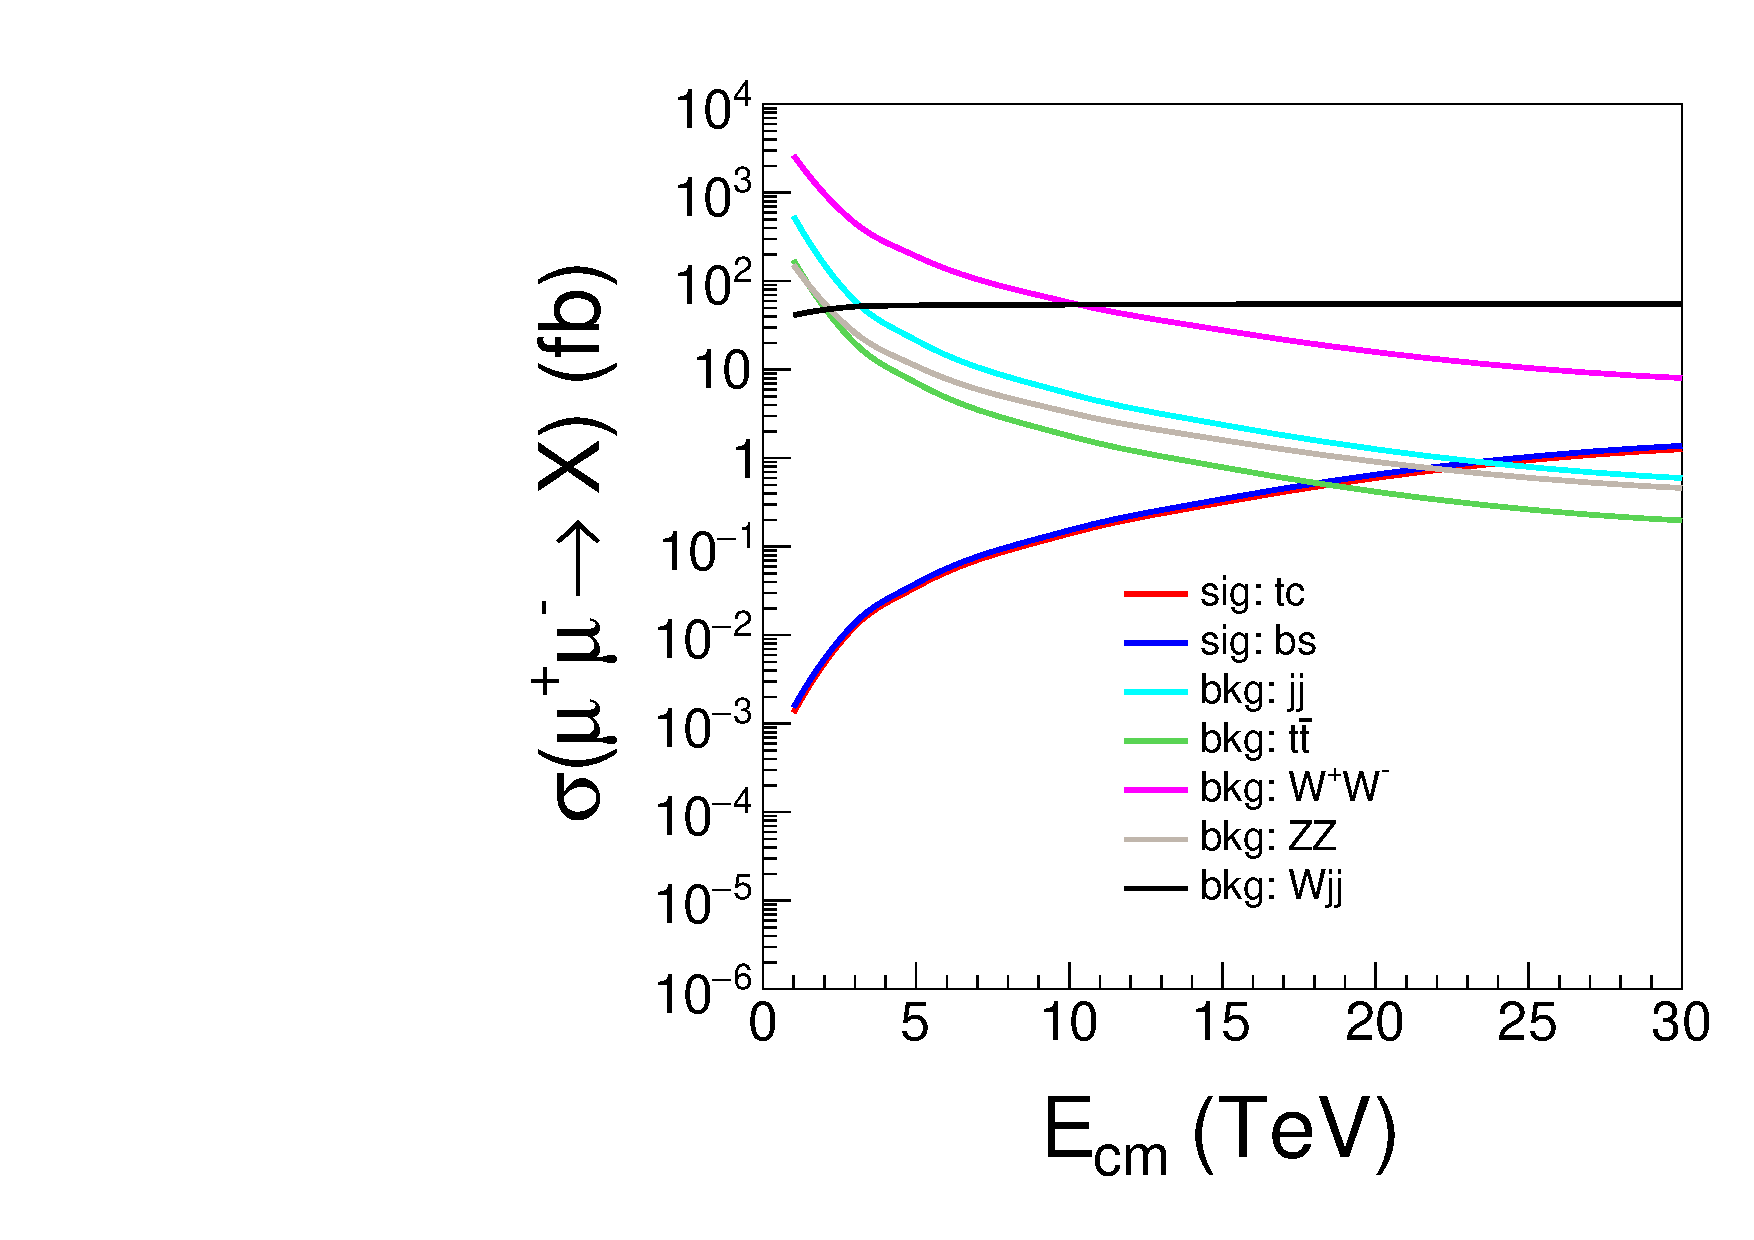
\includegraphics[width=.4\linewidth]{e_sigma_clq1_only.pdf}}
  \subfigure{
  \thesubfigure
  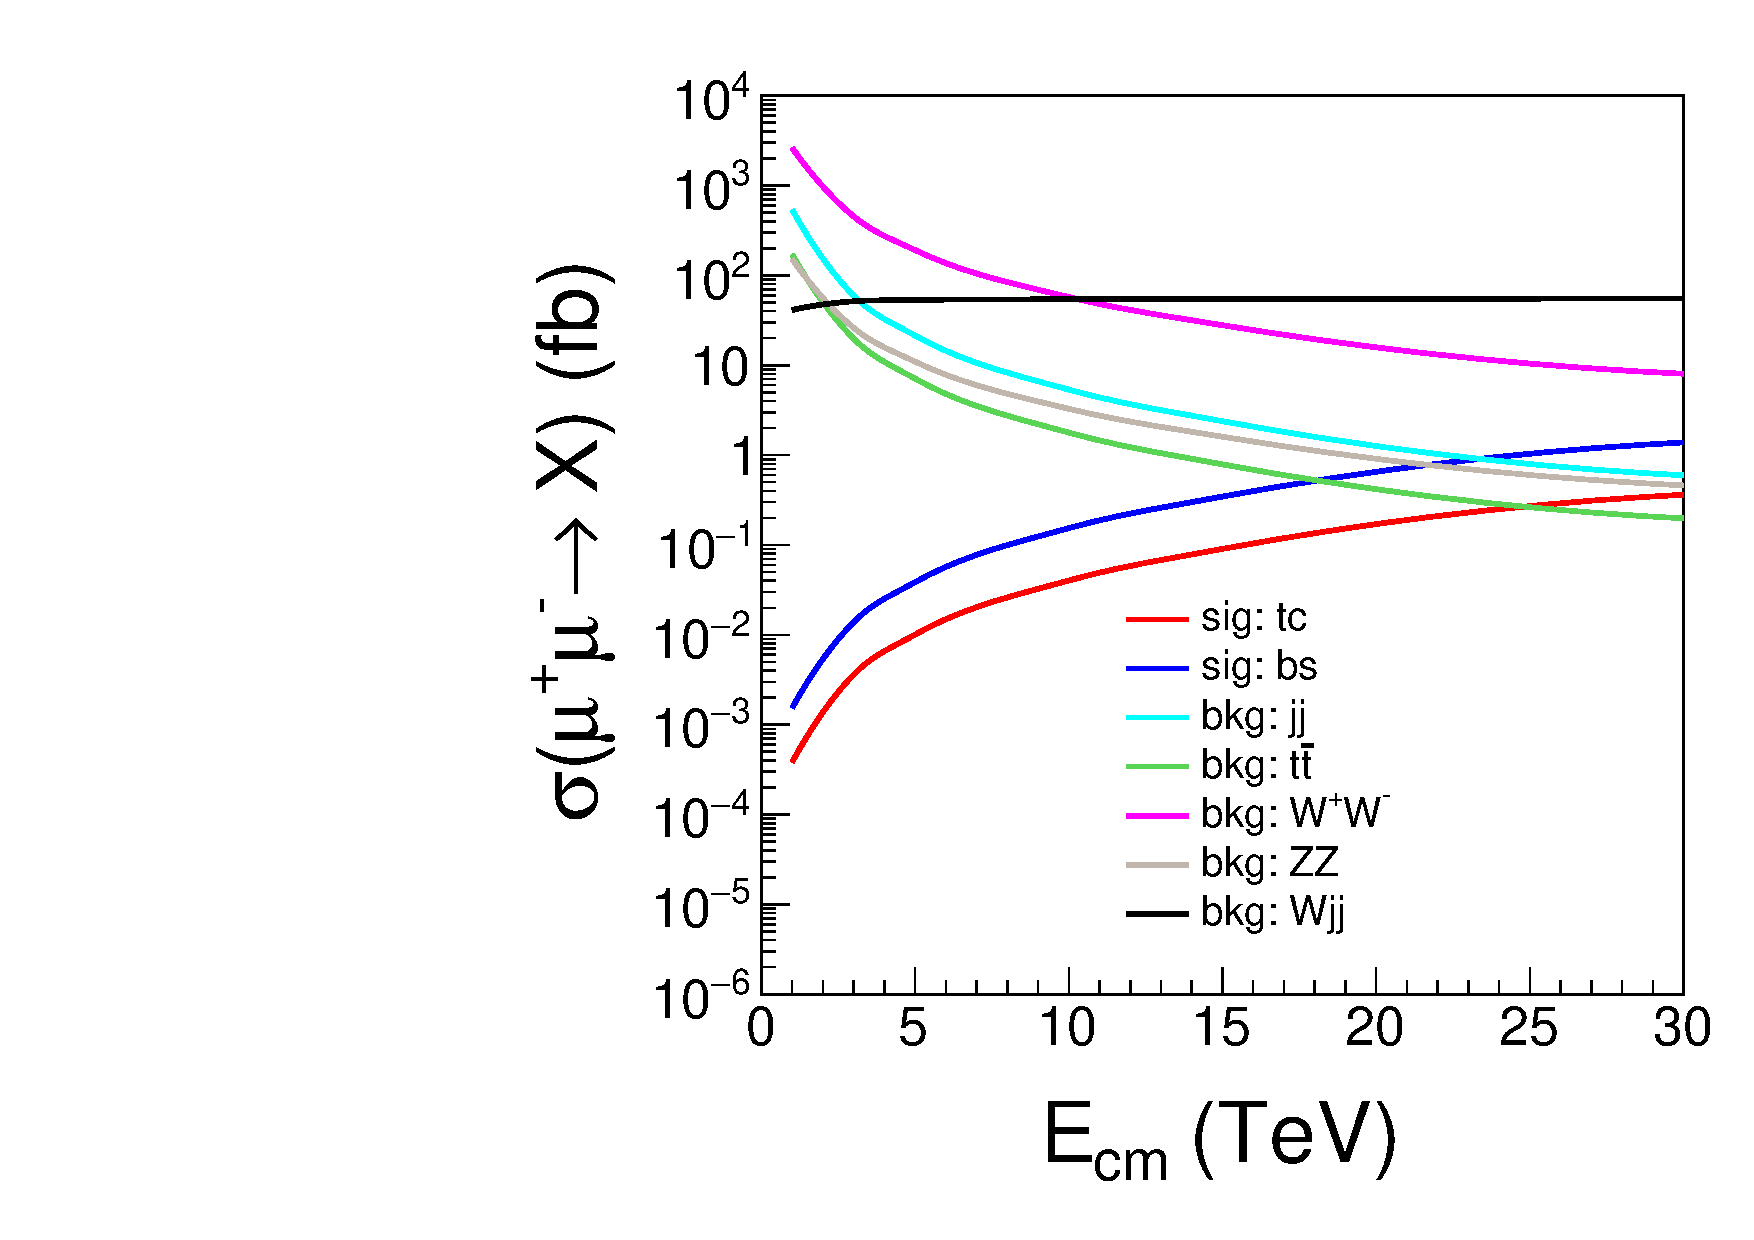
\includegraphics[width=.4\linewidth]{e_sigma_clq1_eq_3clq3.pdf}}
  \caption{The energy dependencies of the cross sections of $\mu^+\mu^-\to X$ are displayed. For the signal, $X=t\bar{c}$, while $X$ is the final state of the background. The best fits $c_{9}=-c_{10}=-0.39$ in Ref.~\cite{Altmannshofer:2021qrr} have been considered here. Their values are evaluated to the cutoff $\Lambda=10$ TeV by our RGEs and matching conditions in the Appendix. Two relations between $C^{(1)}_{lq}$ and $C^{(3)}_{lq}$ have been considered: (a) $C^{(1)}_{lq}=L^{V,LL}_{ed}\times \Lambda^2/v^2$ and $C^{(3)}_{lq}=0$, and (b) $C^{(1)}_{lq}=3C^{(3)}_{lq}=\frac{3}{4}L^{V,LL}_{ed}\times \Lambda^2/v^2$.\label{ecm}}
\end{figure}

In Fig.~\ref{ecm}, the best fits of $c_{9}$ and $c_{10}$ in Ref.~\cite{Altmannshofer:2021qrr} have been considered. 
Their values are evaluated to the EW scale by our RGEs Eq.~\ref{beta:VLLed} and Eq.~\ref{beta:VLRde}. 
And then they are matched to SMEFT by Eq.~\ref{match:VLLed} and Eq.~\ref{match:VLRde}. 
From Eq.~\ref{match:VLLed}, we also know that the constraint from B physics can be only applied to the sum of $C^{(1)}_{lq}+C^{(3)}_{lq}$~\footnote{The generation indices are always $(p,r,s,t)=(2,2,2,3)$ for $C^{(1)}_{lq}$ and $C^{(3)}_{lq}$ and $(p,r,s,t)=(2,3,2,2)$ for $C_{qe}$ in this paper}.  
So any new physics scenarios with $C^{(1)}_{lq}$ and $C^{(3)}_{lq}$ as free parameters cannot be constrained by the data from B physics experiments. 
In Fig.~\ref{rge:EWtoUV}, we show the running of $C^{(1)}_{lq}+C^{(3)}_{lq}$ and $C_{qe}$ from EW scale to new physics scale at $\Lambda=10$ TeV, 
in the case of $c_{9}=-0.73$ and $c_{10}=0$.
We have considered three naive scenarios: 1) $C^{(1)}_{lq}=L^{V,LL}_{ed}\Lambda^2/v^2$, 2) $C^{(3)}_{lq}=L^{V,LL}_{ed}\Lambda^2/v^2$, and 3) $C^{(1)}_{lq}=C^{(3)}_{lq}=L^{V,LL}_{ed}\Lambda^2/2v^2$.
Obviously, it is hard to distinguish these three cases. 

\begin{figure}
  \centering
  \subfigure{
  \thesubfigure
  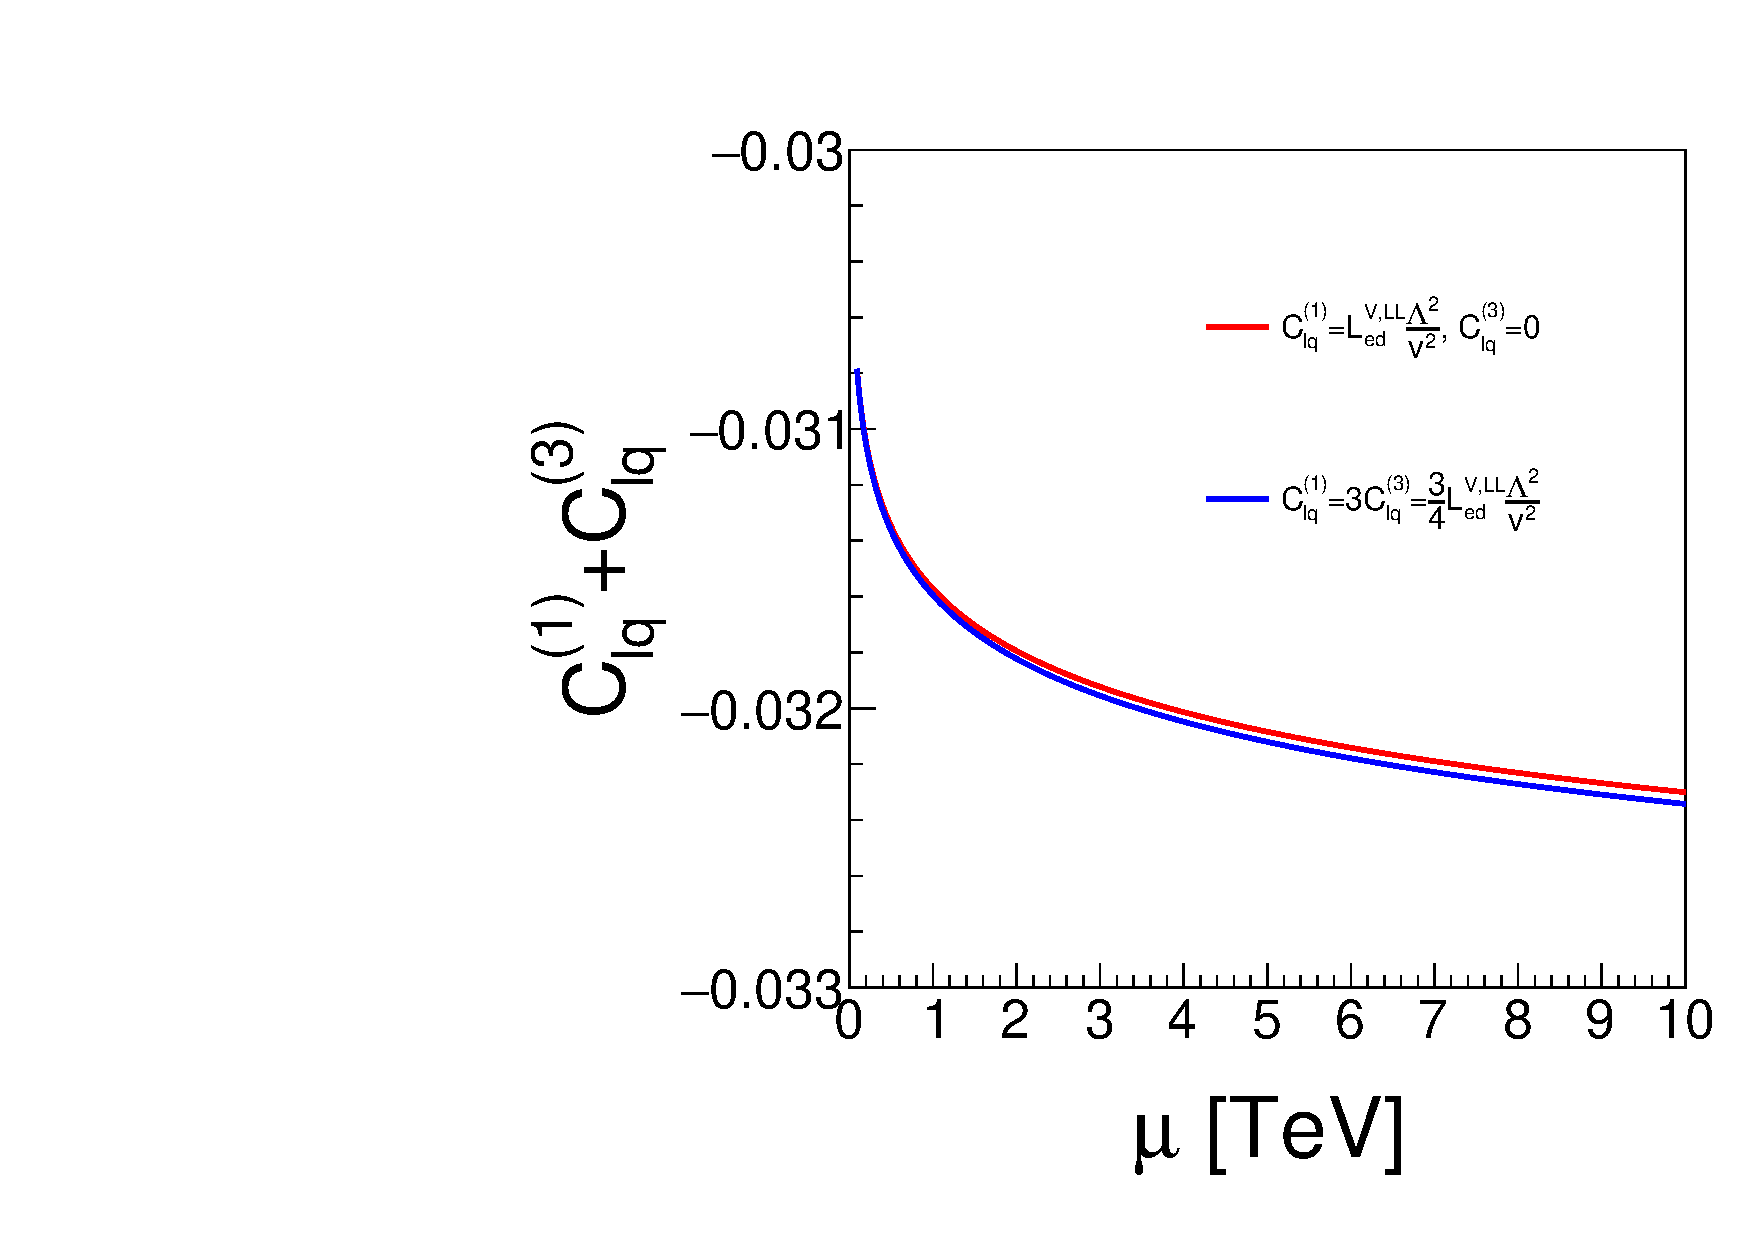
\includegraphics[width=.4\linewidth]{output_plus.pdf}}
  \subfigure{
  \thesubfigure
  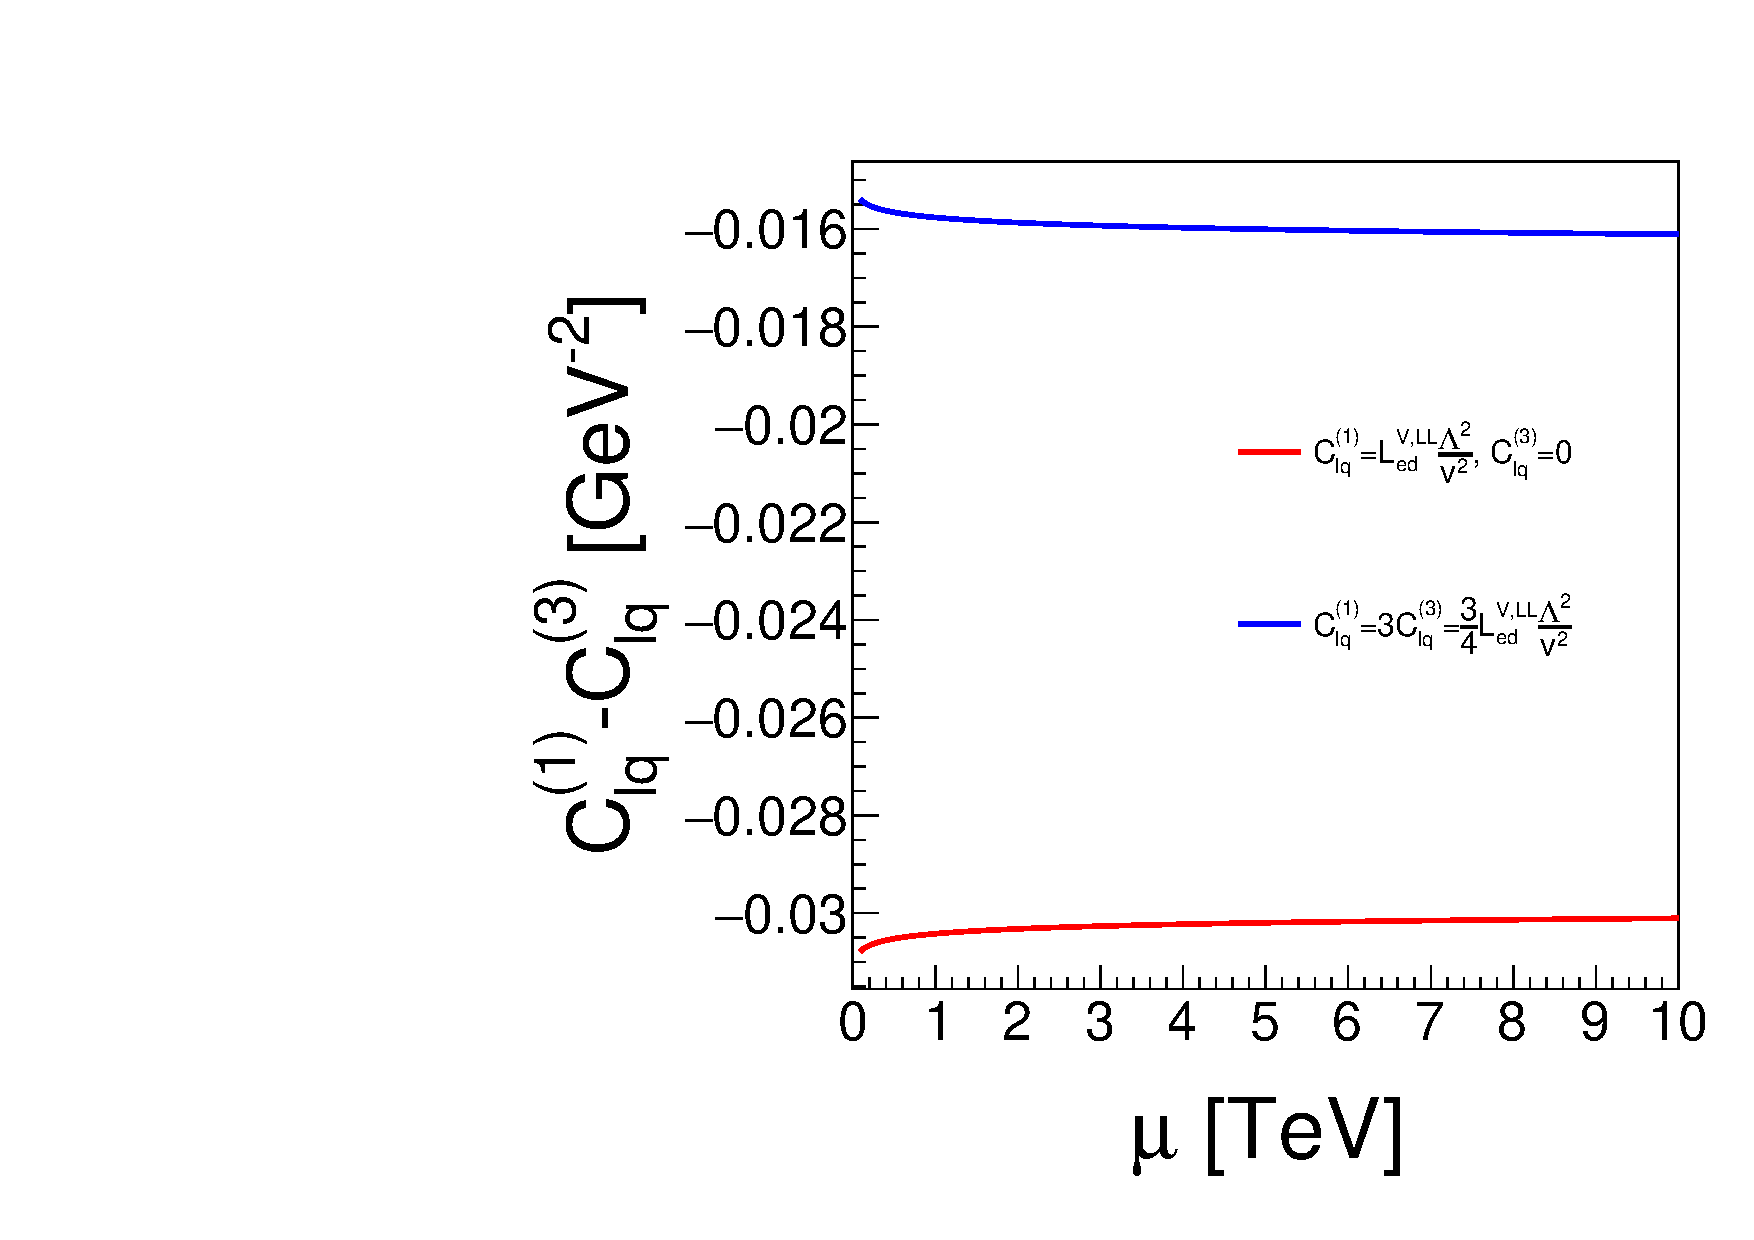
\includegraphics[width=.4\linewidth]{output_minus.pdf}}
  \caption{The running of (a) $C^{(1)}_{lq}+C^{(3)}_{lq}$ and (b) $C^{(1)}_{lq}-C^{(3)}_{lq}$ from EW scale to $\Lambda=10$ TeV is display.  Two scenarios: 1) $C^{(1)}_{lq}=L^{V,LL}_{ed}\Lambda^2/v^2$ and $C^{(3)}_{lq}=0$, and 2) $C^{(1)}_{lq}=3C^{(3)}_{lq}=\frac{3}{4}L^{V,LL}_{ed}\times \Lambda^2/v^2$ have been considered here.\label{rge:EWtoUV}}
\end{figure}

As we have seen in Fig.~\ref{ecm}, the process $\mu^+\mu^-\to t\bar{c}$ can only be observable when $E_{cm}>10$ TeV.  
In such high energy, we can expect that two energetic jets are observed at the detector for either signal and background events. 
For the signal events, one jet with invariant mass around top mass and another one with invariant mass around charm mass~\footnote{In our Monte Carlo simulation, the charm mass is set to zero}. 
While for other background events, such as $W^+ W^-$ and $t \bar{t}$, the invariant mass of boosted W and top quark can generate large jet mass when the cone parameter is large enough to include all their decay products.
For background events, such as $j j$, we expect jet mass should be small if the jet cone parameter is set to be appropriate.

To further investigate the kinematic features of signal, 
we use PYTHIA8~\cite{Bierlich:2022pfr} for parton shower and hadronization, 
and FastJet~\cite{Cacciari:2011ma} to reconstruct jets.  
In the FastJet, we use the generalised $k_t$ algorithm~\cite{Catani:1991hj} for $e^+e^-$ collisions. 
This algorithm defines two distances:
\begin{eqnarray}
  d_{ij} &=& \min(E^{2p}_i,E^{2p}_j)\frac{1-\cos\theta_{ij}}{1-\cos{R}} \nonumber \\
  d_{iB} &=& E^{2p}_i \nonumber 
\end{eqnarray}
where $p$ and $R$ are input by user. If a $d_{ij}$ is smallest then particle $i$ and $j$ are recombined, while $d_{iB}$ is smallest then $i$ is called an ``inclusive jet''.
In this context, we choose $p=1$.

To optimized the value of $R$, we plot the invariant masses of the heaviest jet and the second heaviest jet with different $R$ parameters in Fig.~\ref{sig:mj1} and Fig.~\ref{sig:mj2}, respectively.
The collision energy of these figures are fixed to $10$ TeV, and we require these jets have energy $E>500$ GeV. 
The signal events are generated with $c_{9}=-0.73$ and $c_{10}=0$.
Obviously, we can see that the invariant mass of the heaviest jet has a peak around top mass when $R\geq 0.07$.  
A small peak around $W$ mass is also appeared when $R\leq 0.09$
For the second heaviest jet, we can also see a small peak when $R\geq 0.10$. 
This means that the QCD radiations at the $10$ TeV muon collider can be very energetic. 
Such kind of high energy radiations are collected to be a heavy jet with invariant mass larger than top quark. 
So we can conclude that the best $R$ for signal should be $0.09$ or $0.10$.

\begin{figure}[htbp]
%  \setcounter{subfigure}{0}
  \centering
  % Requires \usepackage{graphicx}
  \subfigure{
  \thesubfigure
  \label{sig:mj1:R005to009}
  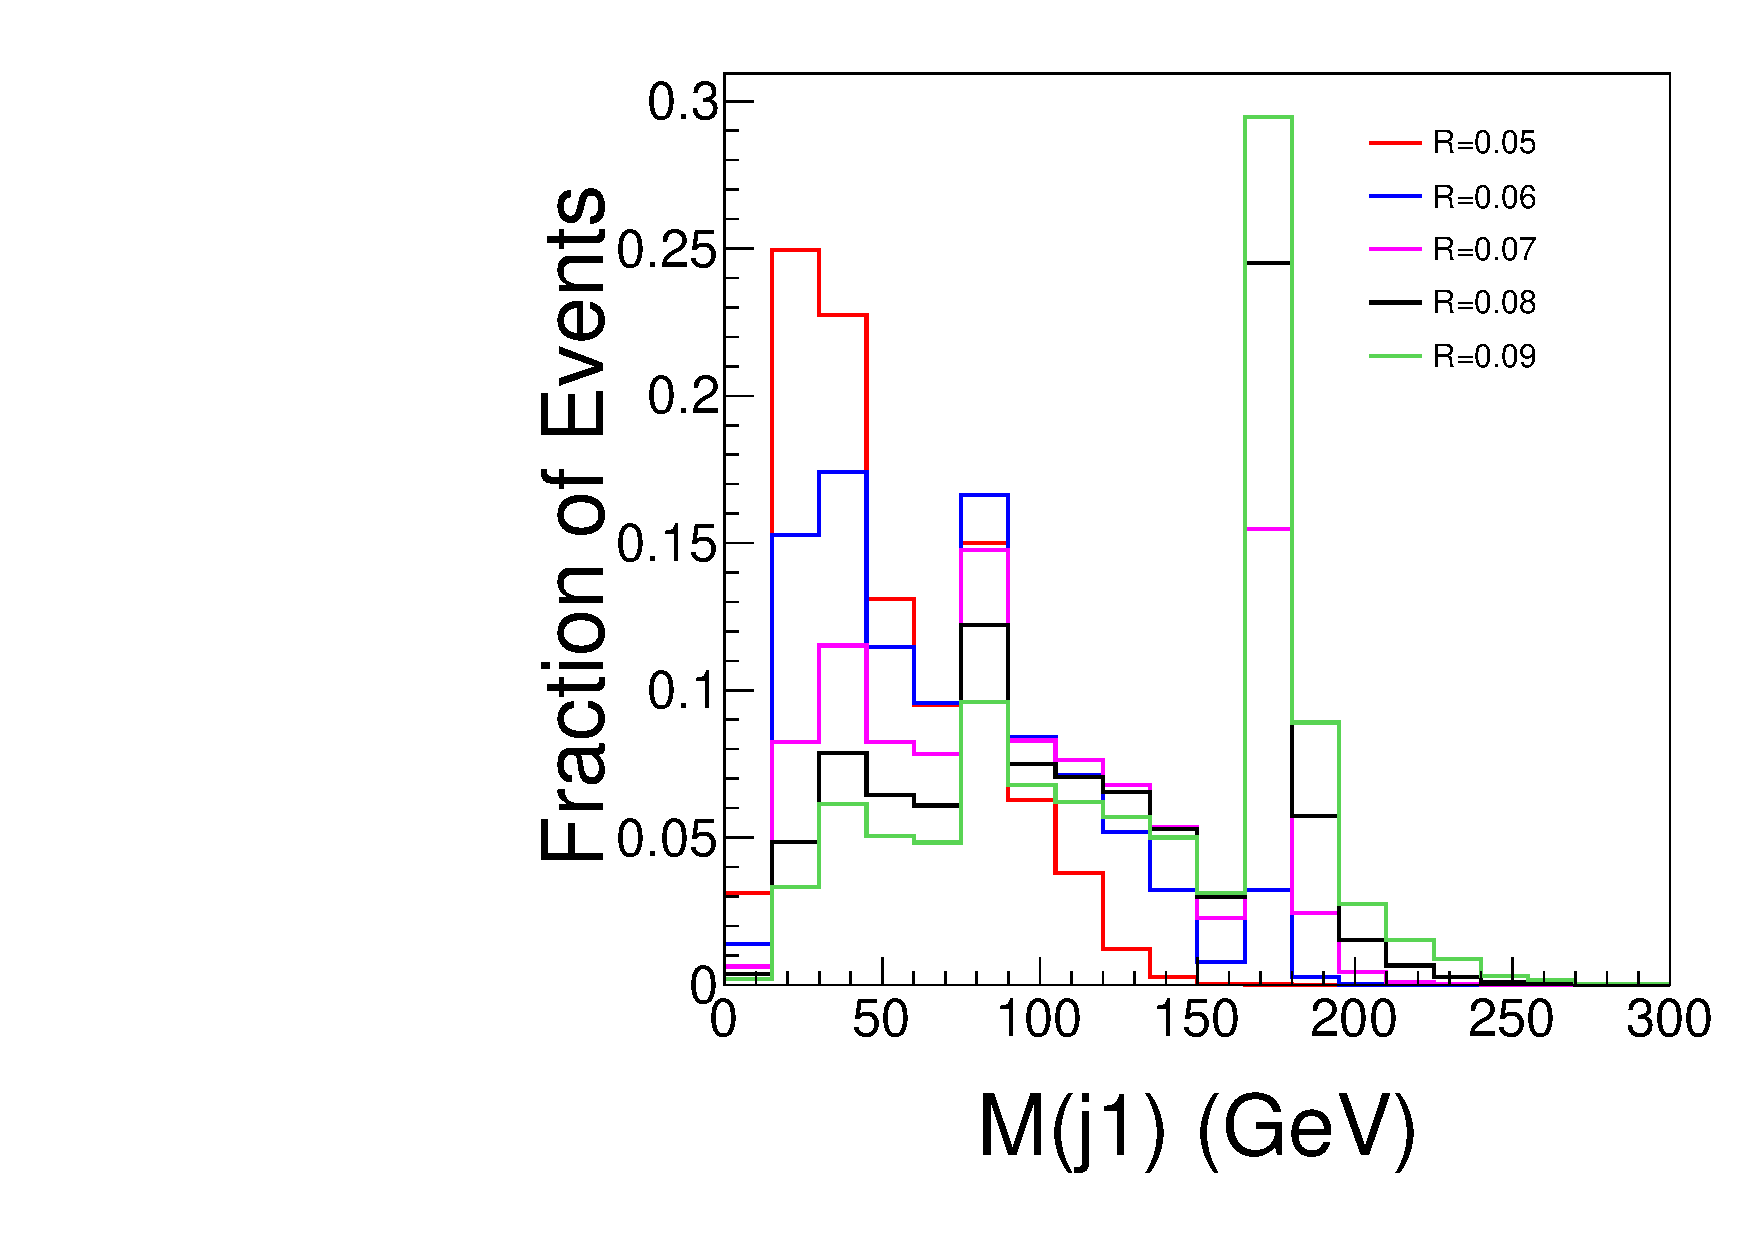
\includegraphics[width=0.4\textwidth]{mj1_clq1only_R005to009.pdf}}
  \subfigure{
  \thesubfigure
  \label{sig:mj1:R010to014}
  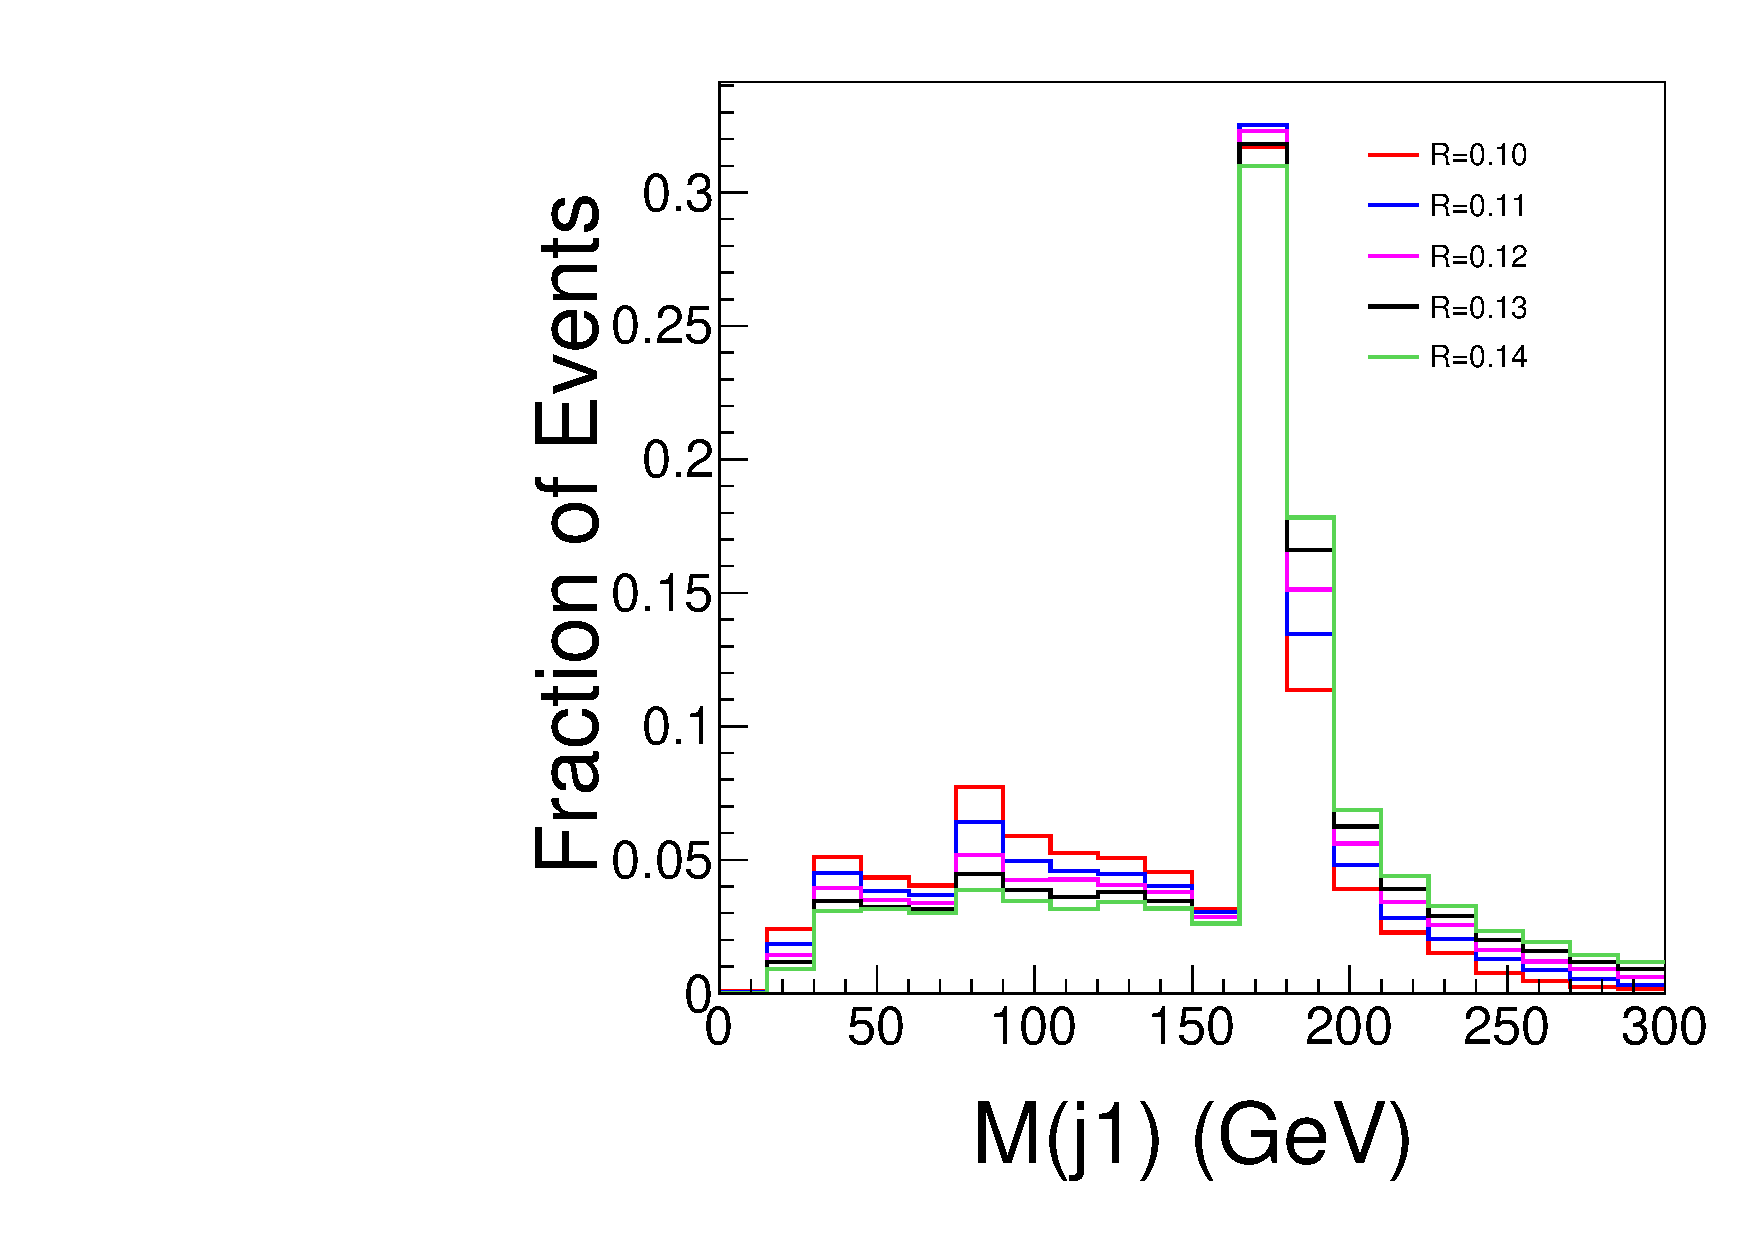
\includegraphics[width=0.4\textwidth]{mj1_clq1only_R010to014.pdf}}
  \caption{The invariant mass of the heaviest jet in the process $\mu^+\mu^-\to t\bar{c}$. In (a), the $R$ is set from $0.05$ to $0.09$, while (b) is set from $0.10$ to $0.14$.}\label{sig:mj1}
\end{figure}

\begin{figure}[htbp]
%  \setcounter{subfigure}{0}
  \centering
  % Requires \usepackage{graphicx}
  \subfigure{
  \thesubfigure
  \label{sig:mj2:R005to009}
  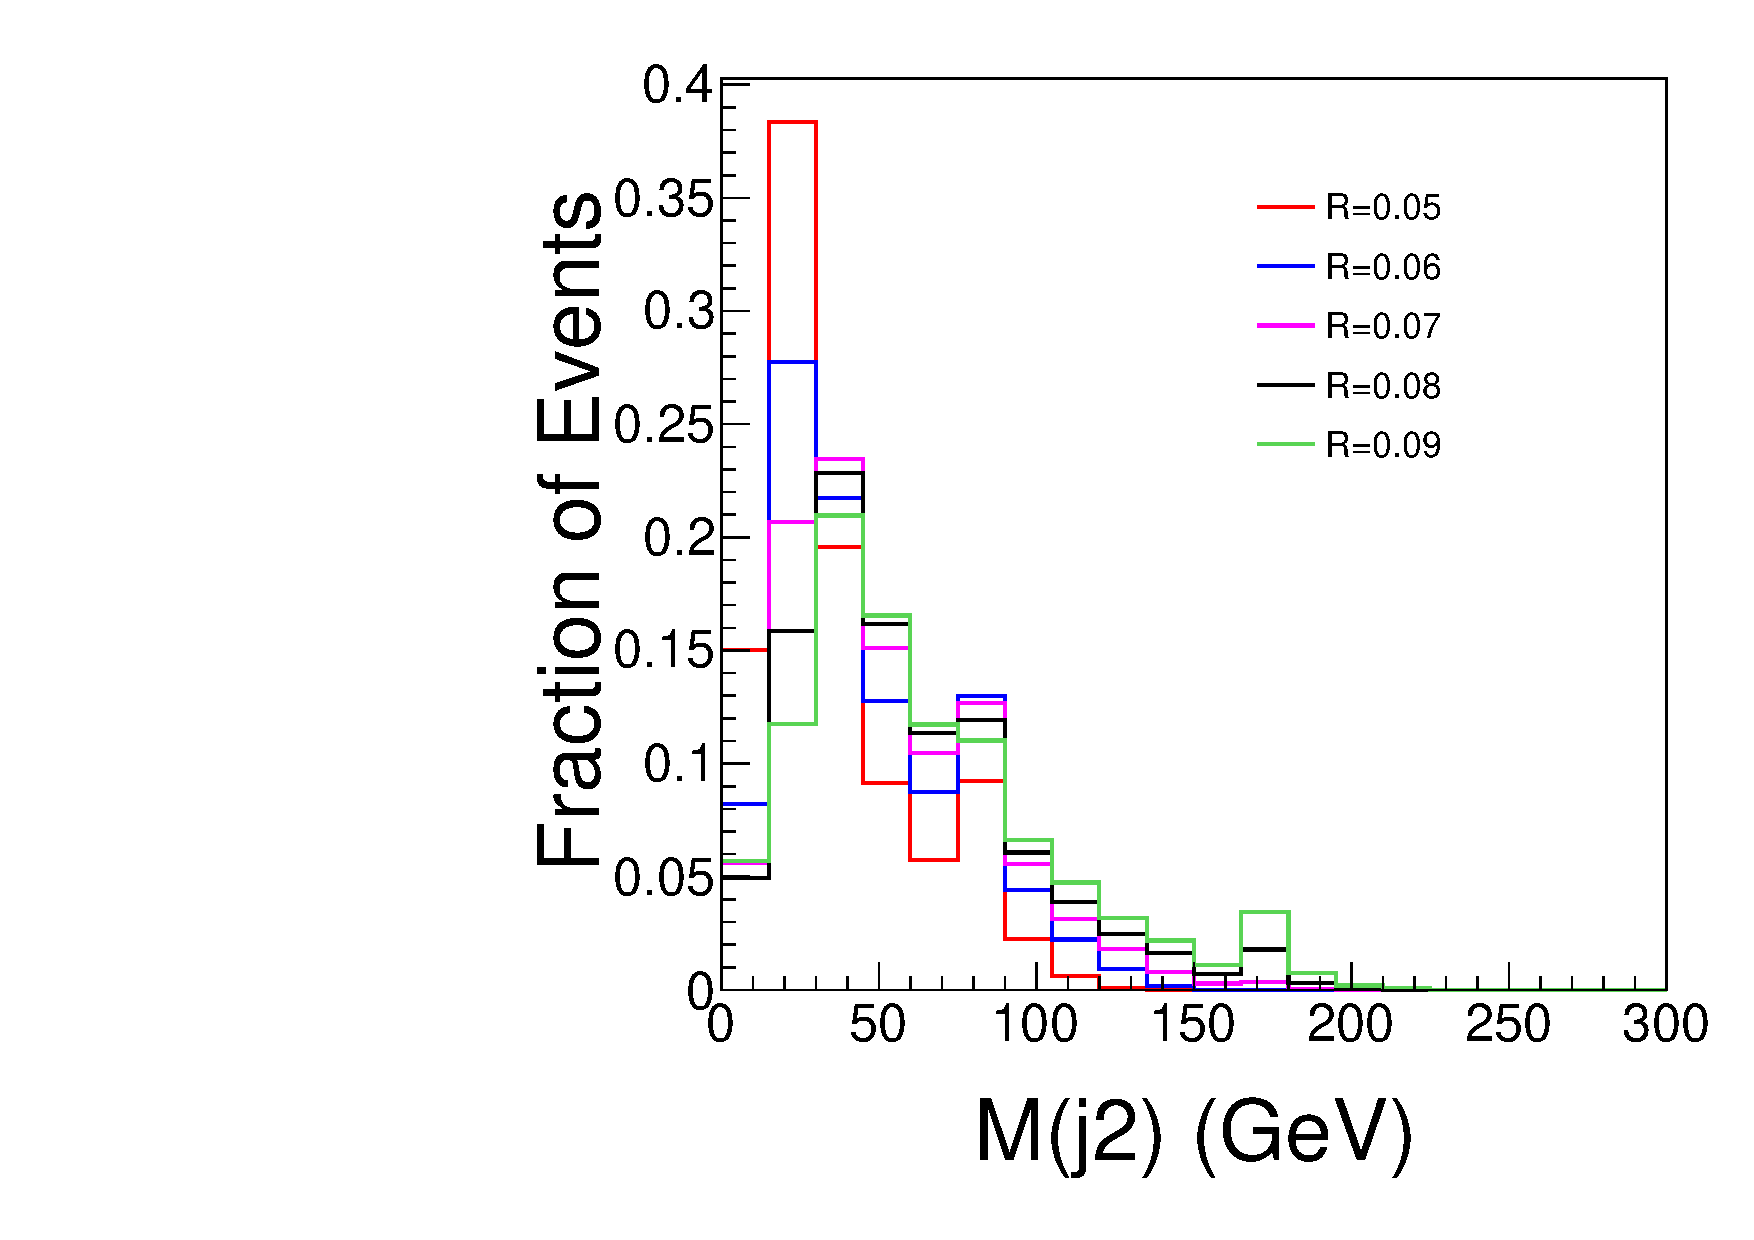
\includegraphics[width=0.4\textwidth]{mj2_clq1only_R005to009.pdf}}
  \subfigure{
  \thesubfigure
  \label{sig:mj2:R010to014}
  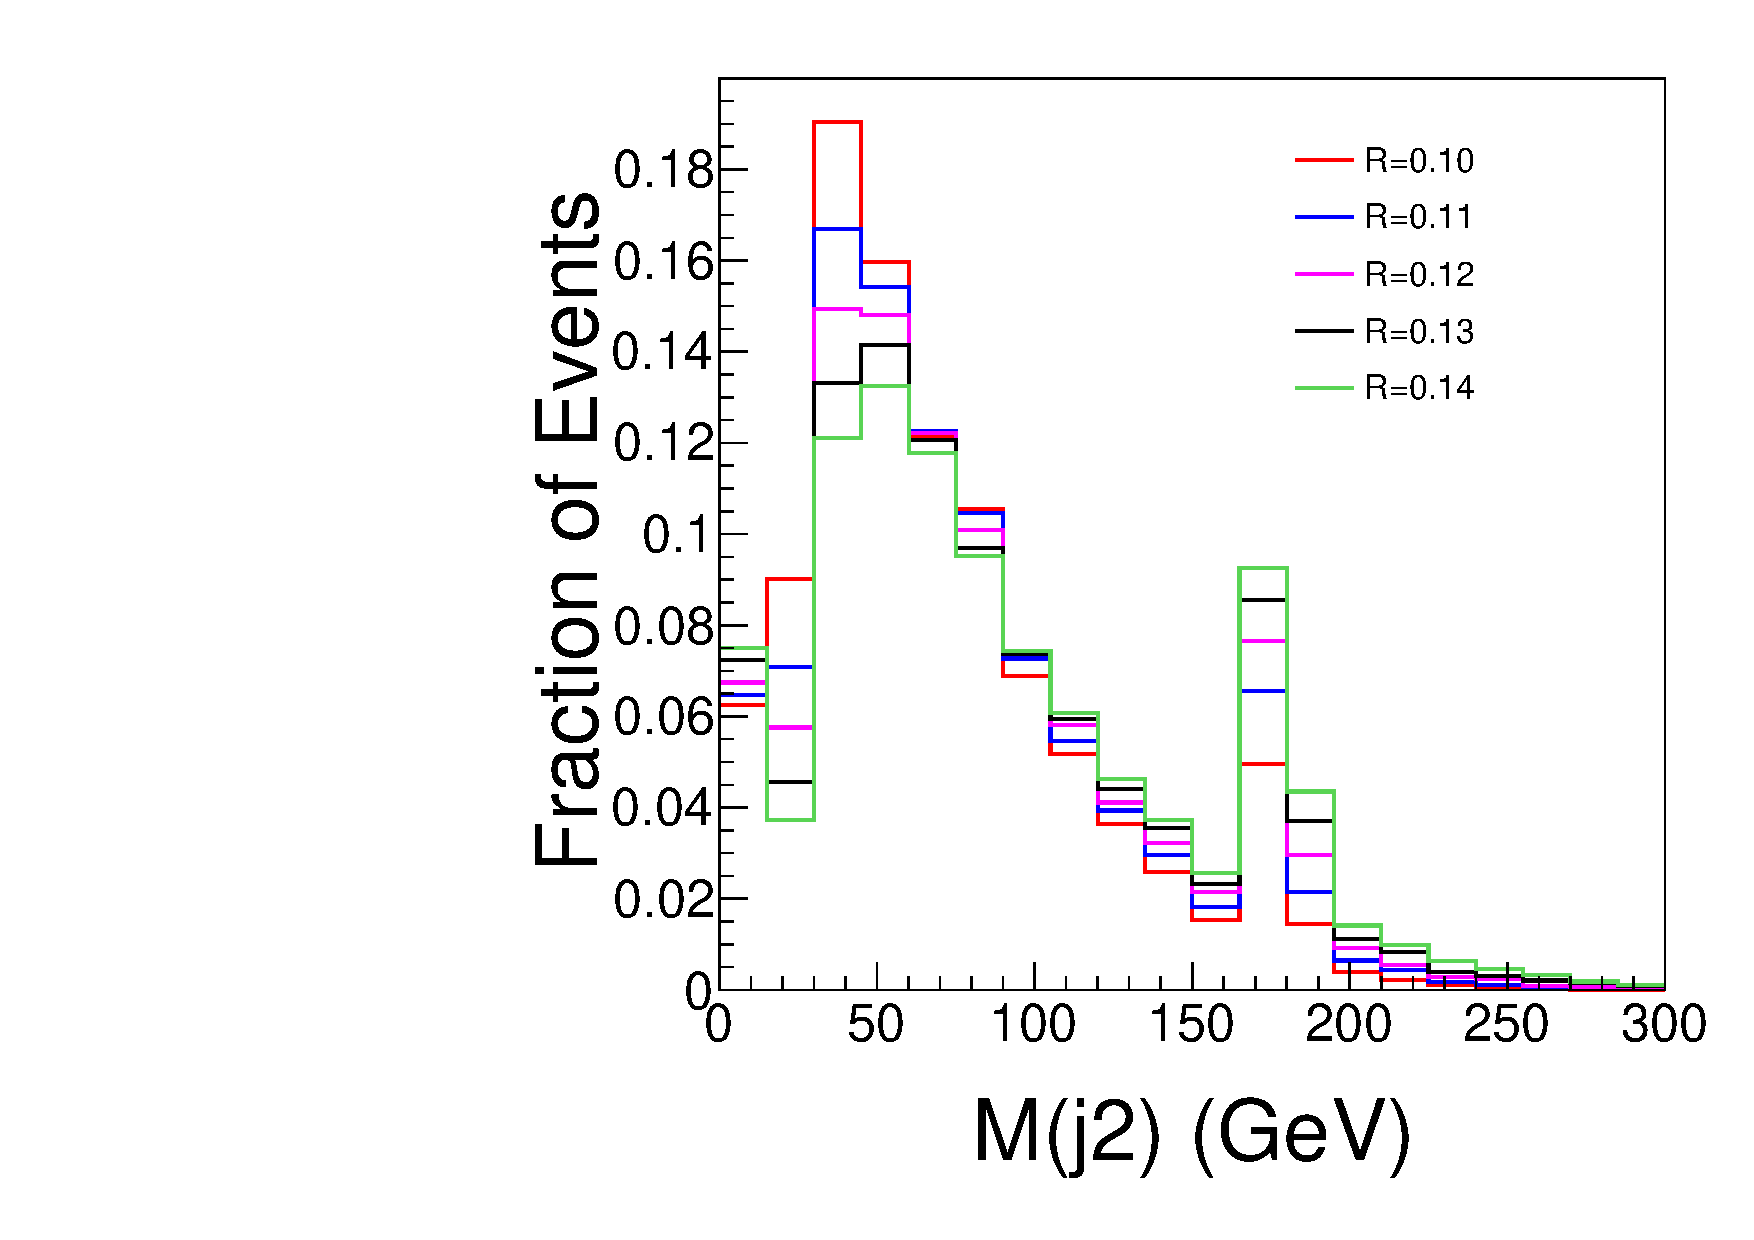
\includegraphics[width=0.4\textwidth]{mj2_clq1only_R010to014.pdf}}
  \caption{The invariant mass of the heaviest jet in the process $\mu^+\mu^-\to t\bar{c}$. In (a), the $R$ is set from $0.05$ to $0.09$, while (b) is set from $0.10$ to $0.14$.}\label{sig:mj2}
\end{figure}

The background $\mu^+\mu^-\to t\bar{t}$ should have similar features in these distributions. 
Fig.~\ref{mj1mj2} shows the invariant masses of the two heaviest jets of $t\bar{t}$ background. 
As we expect, when the jet cone parameter is set to be $R=0.1$, there are large fraction of events which can have two peaks around top mass. In contrast, for the signal events, only one jet can have a jet mass around top mass.

A simple cut to separate signal and background events was demonstrated in Figure 6, where we use the sum of jet mass of two leading massive jets as an observable to separate signal and background events.

The significance for case 1 and case 2.

\begin{figure}[htbp]
  \setcounter{subfigure}{0}
  \centering
  % Requires \usepackage{graphicx}
  \subfigure{
  \thesubfigure
  \label{mj1}
  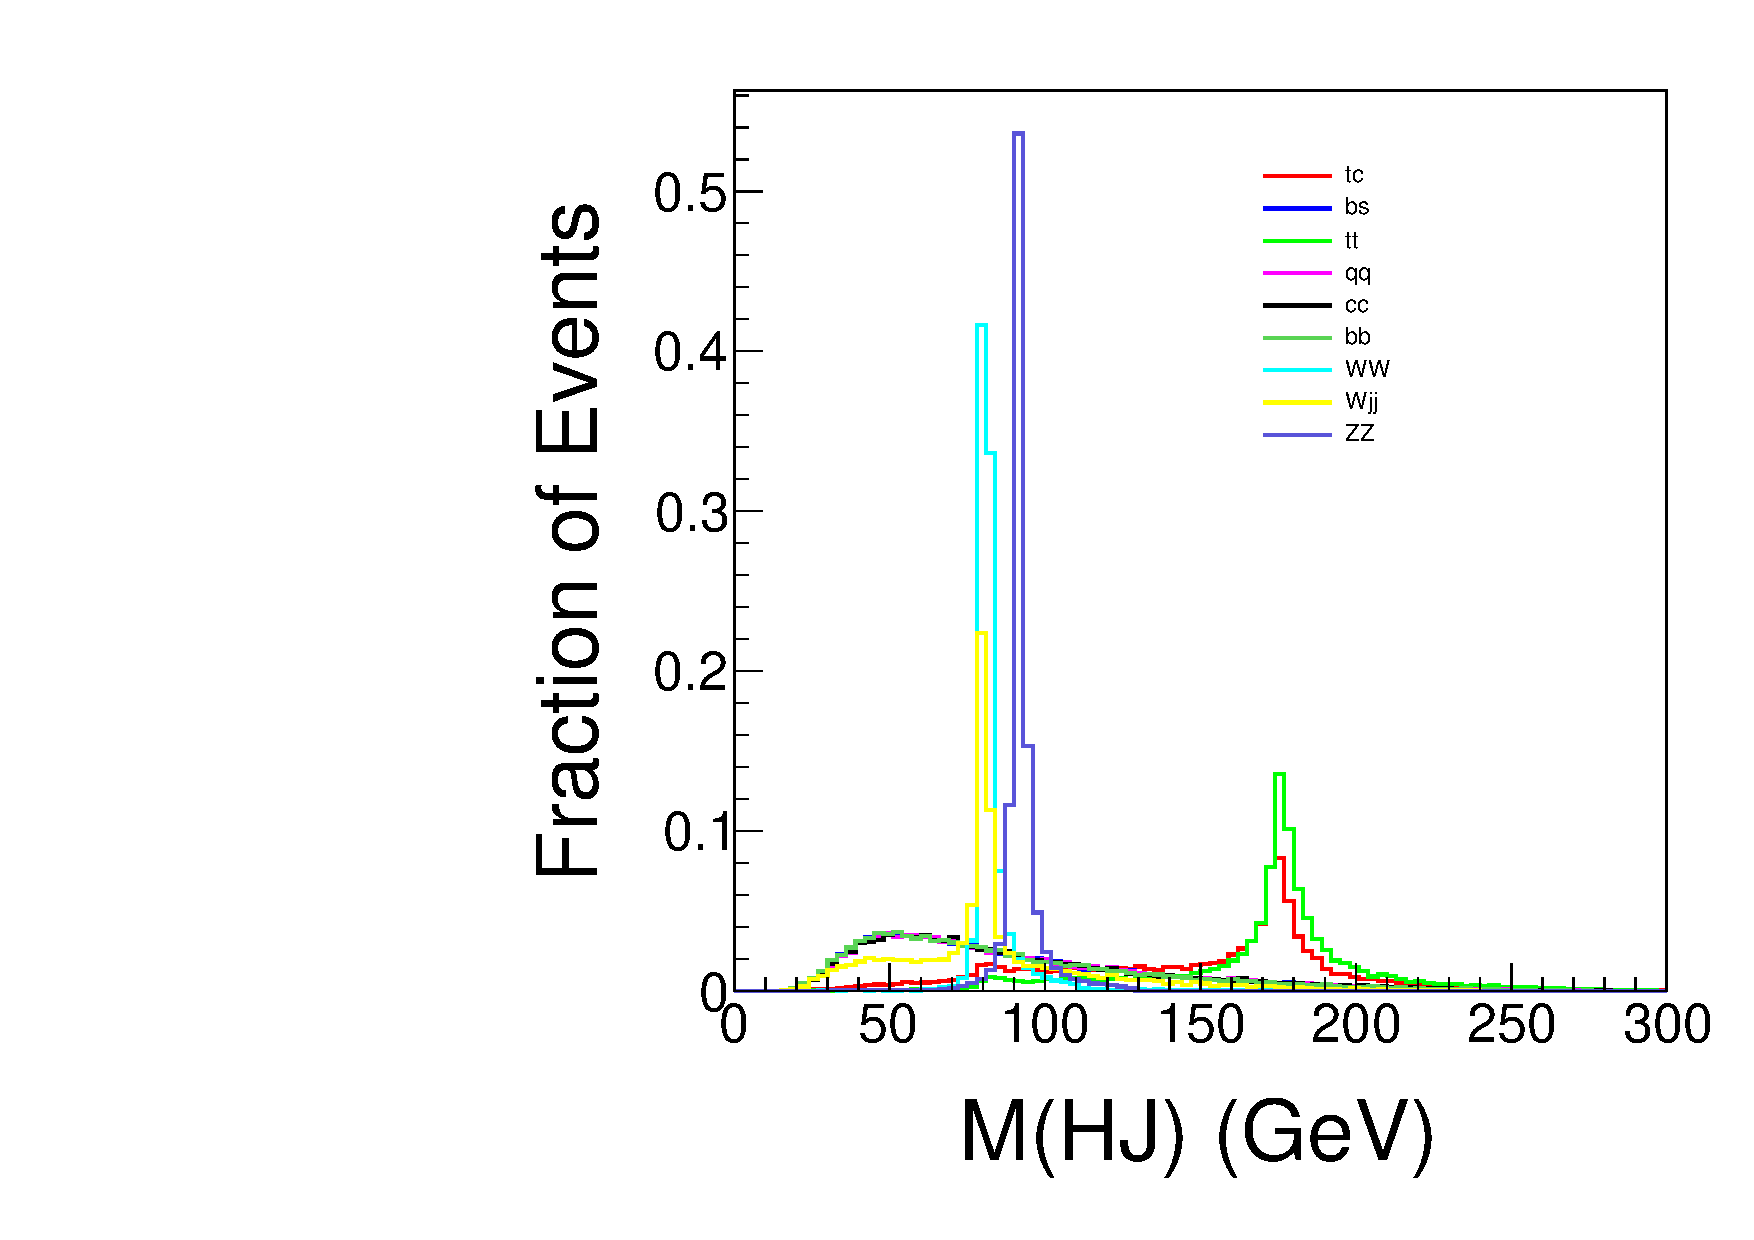
\includegraphics[width=0.4\textwidth]{mj1.pdf}}
  \subfigure{
  \thesubfigure
  \label{mj2}
  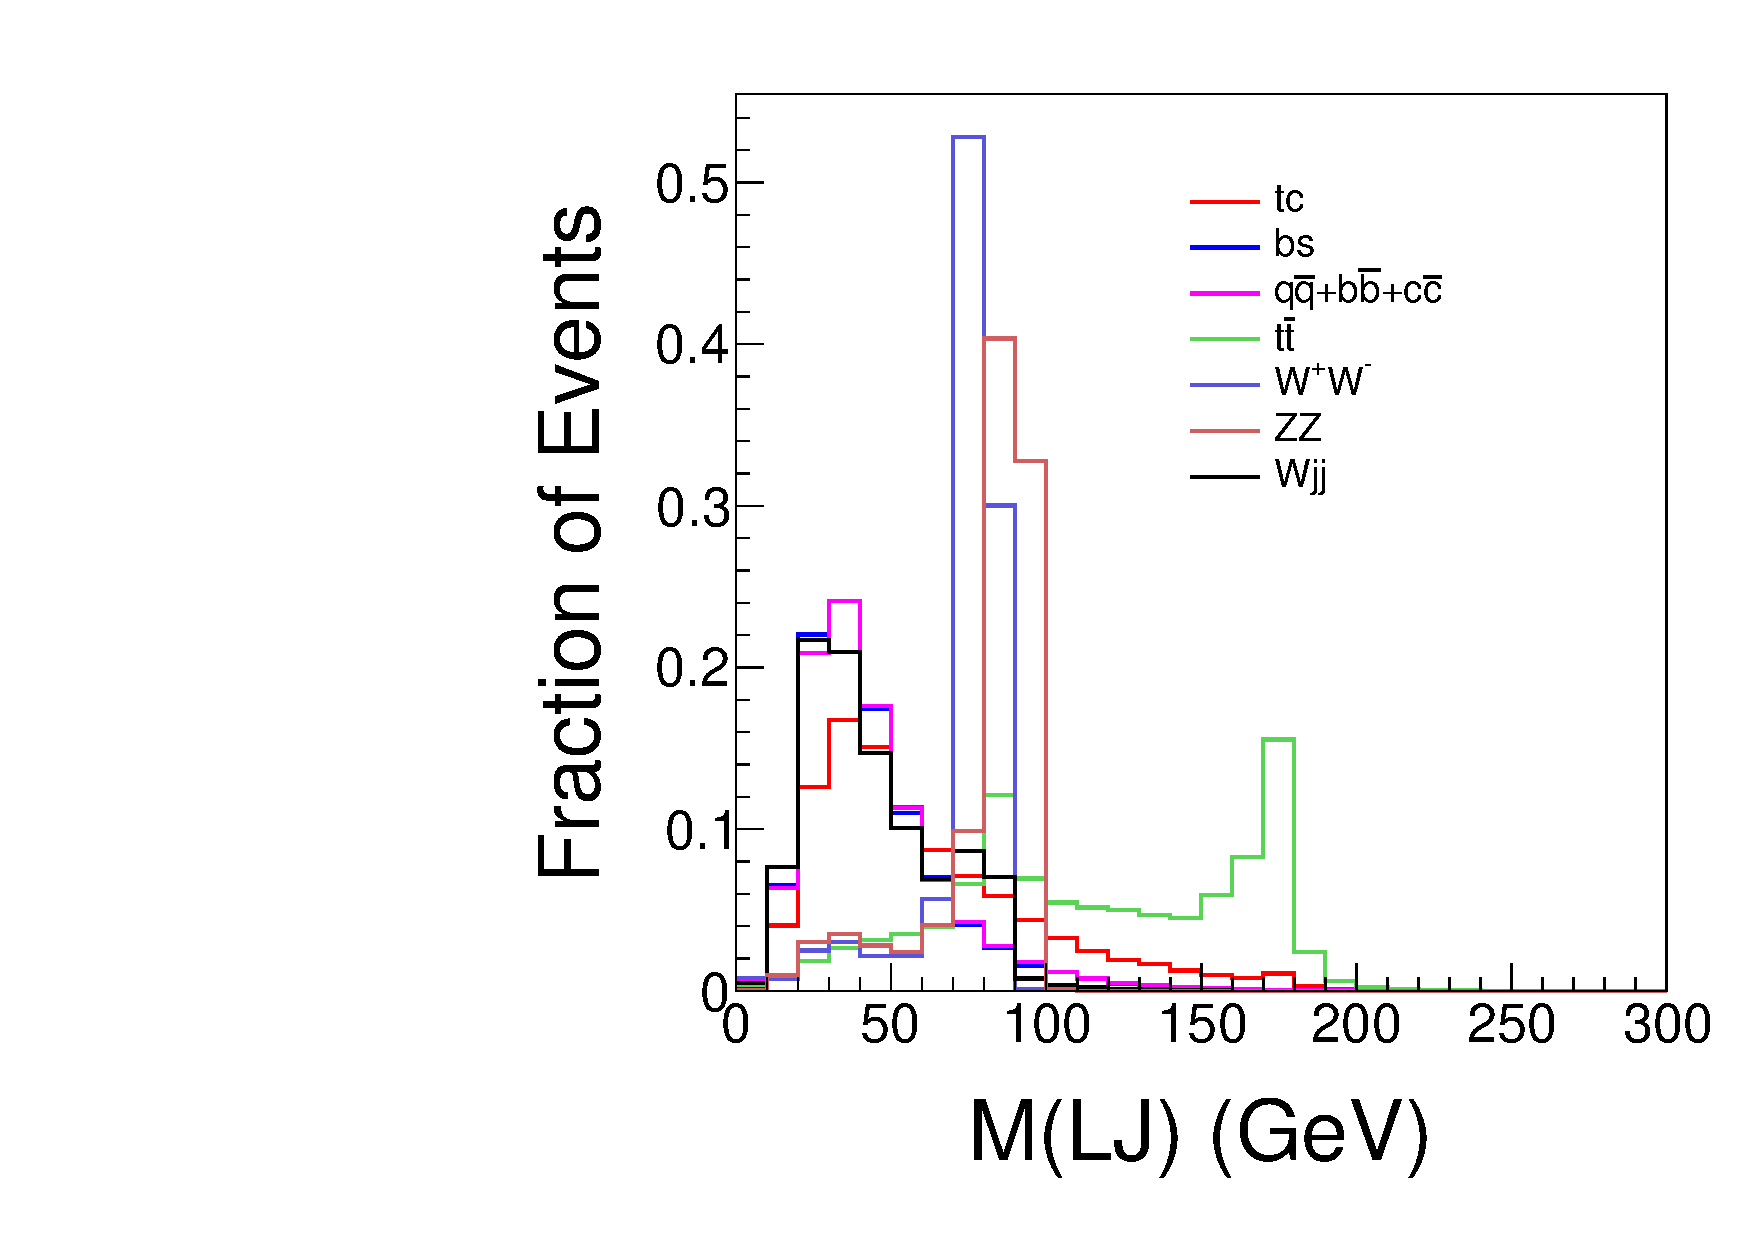
\includegraphics[width=0.4\textwidth]{mj2.pdf}}
  \caption{The invariant mass of (a) the heaviest jet and (b) the sub-heaviest jet in signal and $t\bar{t}$ background are displayed. Here, $R=0.10$.}\label{mj1mj2}
\end{figure}

\begin{figure}
  \centering
  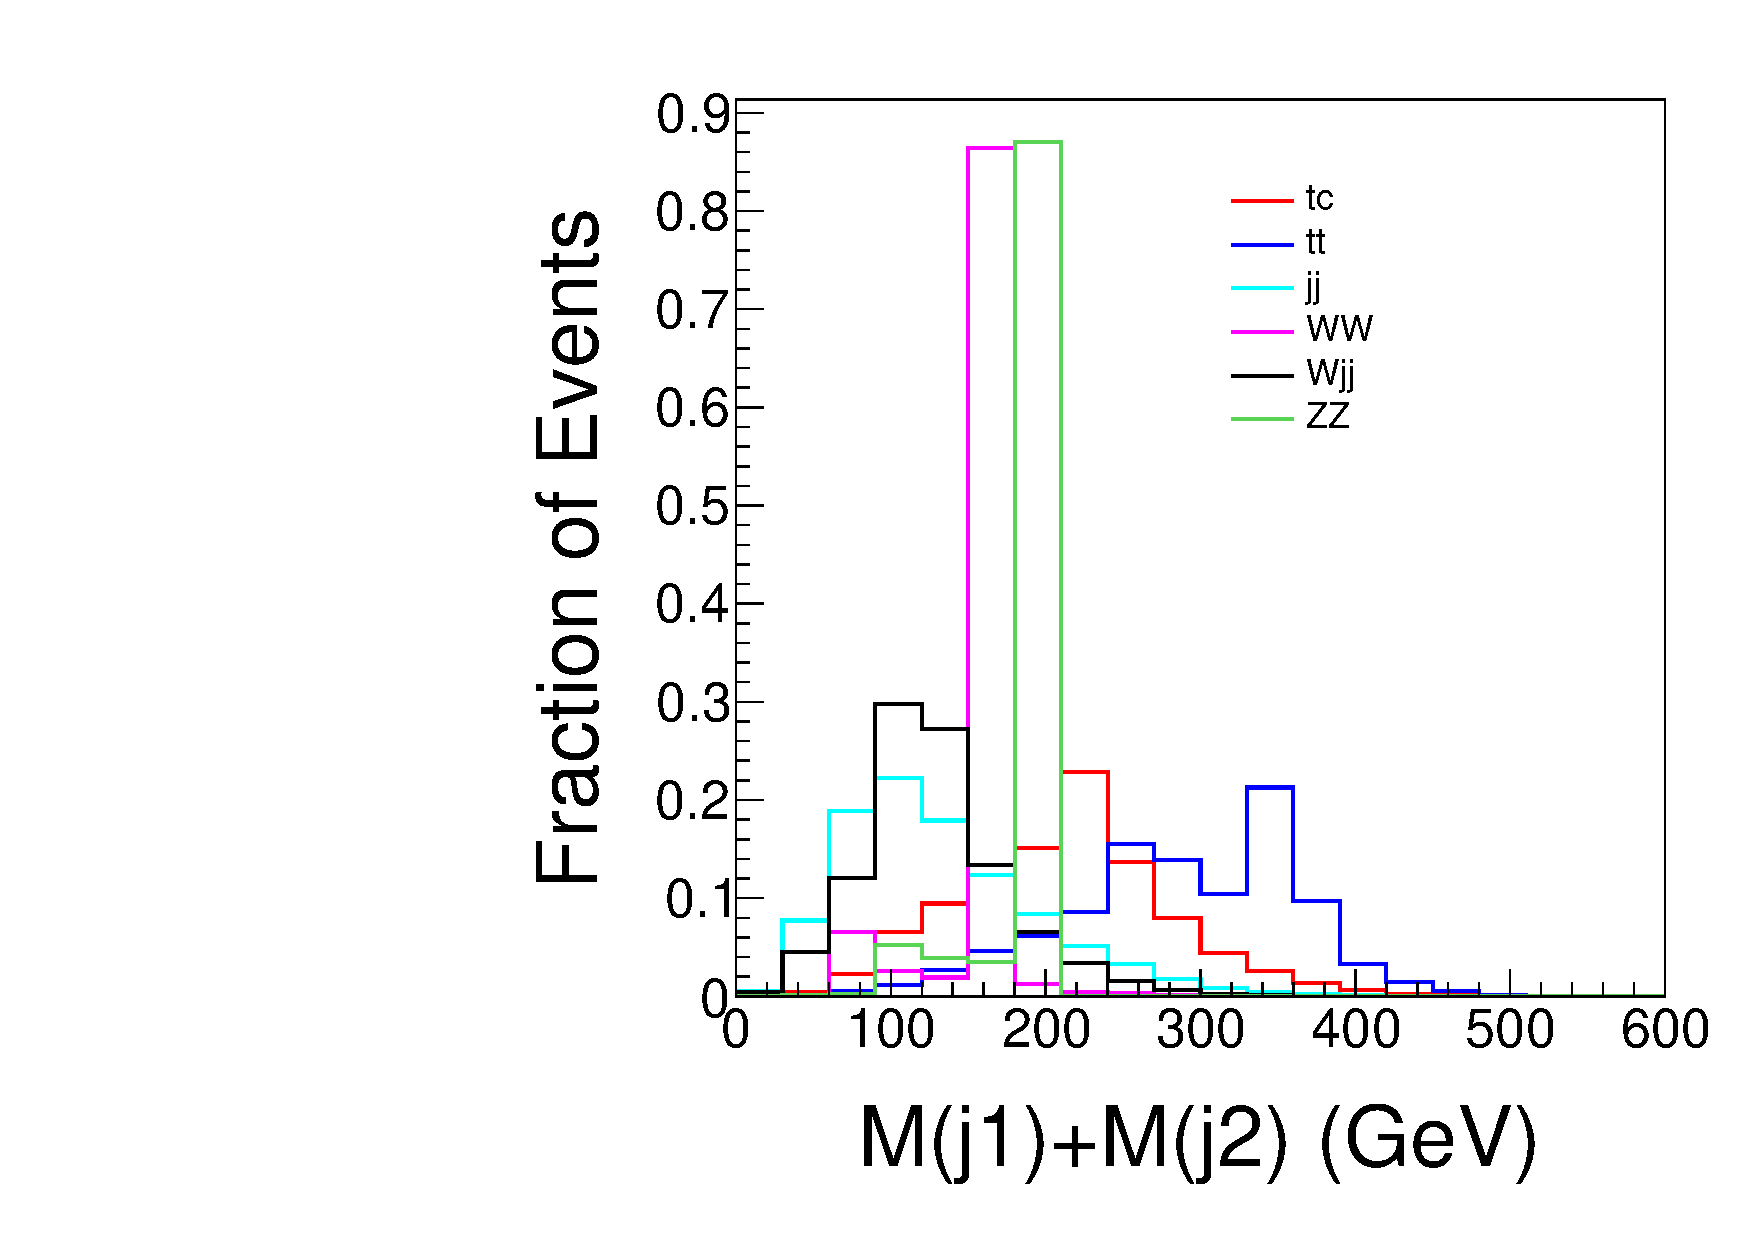
\includegraphics[width=.6\linewidth]{mjsum.pdf}
  \caption{The scale sum of the heaviest and the sub-heaviest jet in signal and backgrounds are displayed. Here, $R=0.10$. \label{mjsum}}
\end{figure}

\begin{center}
\begin{table}
  \begin{center}
  \begin{tabular}{c|c|c}
  \hline
  &  No Cuts   &    $m_t<M(j1)+M(j2)<m_t+m_W$       \\
  \hline
  $\mu^+\mu^-\to tc$     &   4209     &     2085      \\
  $\mu^+\mu^-\to t\bar{t}$     &   $5.343\times{10^4}$      &     $1.100\times{10^4}$     \\
  $\mu^+\mu^-\to jj$     &   $1.607\times{10^5}$      &    $2.890\times{10^4}$        \\
  $\mu^+\mu^-\to W^+W^-$  & $1.723\times{10^6}$   & $4.359\times{10^4}$  \\
  $\mu^+\mu^-\to Wjj$  & $1.628\times{10^6}$   &  $2.177\times{10^5}$ \\
  $\mu^+\mu^-\to ZZ$  & $9.837\times{10^4}$  &  $8.787\times{10^4}$ \\
  \hline
  $S/B$      &  \multicolumn{2}{c}{0.005}  \\
  $S/\sqrt{S+B}$      &  \multicolumn{2}{c}{3.333}  \\
  \hline
  \end{tabular}
  \end{center}
  \caption{The number of events before and after cut are listed. We assume the luminosity is $30$ ab$^{-1}$ at 10 TeV muon collider. \label{table:cut}}
\end{table}
\end{center}

\begin{center}
\begin{table}
  \begin{center}
  \begin{tabular}{c|c|c|c|c|c|c}
  \hline
  &  No Cuts   &    $M(j1)>m_Z$   &  $M(j2)<m_W$  & $n_b=1$ &  $S/B$  &    $S/\sqrt{S+B}$   \\
  \hline
  $\mu^+\mu^-\to tc$     &   4209     &     3193  &     2214  &  1534  &  \multirow{6}{*}{0.164} & \multirow{6}{*}{14.697} \\
  $\mu^+\mu^-\to t\bar{t}$     &   $5.343\times{10^4}$      &     $4.958\times{10^4}$  &  $9487$ & $3984$  & & \\
  $\mu^+\mu^-\to jj$     &   $1.607\times{10^5}$      &    $5.581\times{10^4}$    &  $4.392\times{10^4}$ & $870$ &   &  \\
  $\mu^+\mu^-\to W^+W^-$  & $1.723\times{10^6}$   & $5.445\times{10^4}$ &  $5.238\times{10^4}$ & $1037$ & & \\
  $\mu^+\mu^-\to Wjj$  & $1.628\times{10^6}$   &  $2.906\times{10^5}$   &  $1.664\times{10^5}$ & $3294$  & & \\
  $\mu^+\mu^-\to ZZ$  & $9.837\times{10^4}$  &  $9.557\times{10^4}$   &  $8873$ & $176$  &  & \\
  \hline
%  $S/B$      &  \multicolumn{5}{c}{0.008}  \\
%  $S/\sqrt{S+B}$      &  \multicolumn{5}{c}{4.159}  \\
%  \hline
  \end{tabular}
  \end{center}
  \caption{The number of events before and after cut are listed. We assume the luminosity is $30$ ab$^{-1}$ at 10 TeV muon collider.  The b-tagging efficiency is assumed to be $0.7$ and the fake rate is $0.01$ for light quarks.\label{table:tc:cut}}
\end{table}
\end{center}

\begin{center}
\begin{table}
  \begin{center}
  \begin{tabular}{c|c|c|c|c|c|c}
  \hline
  &  No Cuts  & $N_{jets}<3$  &    $M(j1)<75$ GeV & $n_b=1$ & $S/B$ &  $S/\sqrt{S+B}$  \\
  \hline
  $\mu^+\mu^-\to bs$     &   4599  &  2193   &     971  &  673   &   \multirow{6}{*}{0.631}   &  \multirow{6}{*}{16.134}  \\
  $\mu^+\mu^-\to t\bar{t}$     &   $5.343\times{10^4}$ &   $2.548\times{10^4}$    &  $16$     & $7$ & & \\
  $\mu^+\mu^-\to jj$     &   $1.607\times{10^5}$  &   $7.501\times{10^4}$    &    $3.208\times{10^4}$   &  $635$  & &     \\
  $\mu^+\mu^-\to W^+W^-$  & $1.723\times{10^6}$  &  $1.635\times{10^6}$ &  $3360$ & $67$ & & \\
  $\mu^+\mu^-\to Wjj$  & $1.628\times{10^6}$  &  $4.420\times{10^4}$   &  $1.775\times{10^4}$   &  $351$  & & \\
  $\mu^+\mu^-\to ZZ$  & $9.837\times{10^4}$ & $9.837\times{10^4}$   &  $325$ &  $6$ & &  \\
  \hline
  \end{tabular}
  \end{center}
  \caption{The number of events before and after cut are listed. We assume the luminosity is $30$ ab$^{-1}$ at 10 TeV muon collider.  The b-tagging efficiency is assumed to be $0.7$ and the fake rate is $0.01$ for light quarks.\label{table:bs:cut}}
\end{table}
\end{center}

\section{Summary and Discussion}\label{Sec:conc}
For the signal processes $\mu^+ \mu^- \to b s$ \cite{Altmannshofer:2022xri}, it has been revealed that b tagging is crucial to reject background events from $jj$ final states. The dominant background events are $j j$. In order to extract the information on the Wilson coefficients $C_{9}$ and $C_{10}$, it is found that the polarized muon beams and the measurement of forward-backward asymmetry of final state is crucial. 

In this work, instead of assuming polarized muon beams and charge tagging of final state, we propose to measure the signal processes $\mu^+ \mu^- \to t c$. Then it is found that the major task is to reject $t \bar{t}$ and $ W W$ events, which might be even easier to pick out signal events. It is also found that the weak radiation $ j j W$ is large and might be relevant background.

It is also found that in order to resolve the signal events, detectors with high granuality are needed, since top quarks and W bosons in the hadronic final states are around 5 TeV and are highly boosted objects. In order to capture the substructure of these massive jets, the cone parameter should be set as around  $0.09-0.1$ when the collision energy is assumed to be $\sqrt{s}=10$ TeV, which is much smaller compared with the cone parameter adopted as $R=0.4$ or $0.5$ at the LHC. To extract signal events from large background events, refined analysis of jet substructure at TeV region should be applied in order to achieve a much better performance.

To distinguish new physics models, it is found that the measurement of  $\mu^+ \mu^- \to tc$ can pinpoint the Model I and Model II. Model III can be discovered due to the near resonance near a few TeV region. Model IV could be favored if there is no signal of the process $\mu^+ \mu^- \to t c$ can be measured.

	\begin{acknowledgments}
                Z.J. Zhao has been partially supported by a
		Nikolai Uraltsev Fellowship of the Center for Particle Physics,
		University of Siegen, and partially supported by the Natural Science
		Foundation of China under the grant No. 11875260. 
		S.C. Sun is supported by the MOST of Taiwan
		under grant number of 105-2811-M-002-130 and the CRF Grants of the
		Government of the Hong Kong SAR under HUKST4/CRF/13G.  Q.S. Yan 
		is supported by the Natural Science Foundation of China
		under the grant No.  11475180 and No. 11875260.
		X.R. Zhao has received funding from the European Union's Horizon 2020 research 
		and innovation programme as part of the 
		Marie Sk{\l}odowska-Curie Innovative Training Network MCnetITN3 (grant agreement no. 722104).
		We would like to acknowledge the Mainz Institute for Theoretical Physics(MITP) for enabling us to complete this work.

	\end{acknowledgments}

\appendix
	



\section{SMEFT Renormalization Group Equation}\label{smeftrge}
The RGE of SMEFT Wilson coefficients can be written as 
\begin{eqnarray}
  \frac{dC_i}{d\ln{\mu}} &=& \frac{1}{16\pi^2}\beta_i. \label{beta:definition}
\end{eqnarray}
All 1-loop $\beta$ functions of operators in Warsaw basis have been derived in Ref.~\cite{Celis:2017hod}. 

The $\beta$ functions of operators~\ref{O1lq}$\sim$\ref{Oqe} are
\begin{eqnarray}
   \left[\beta^{(1)}_{lq}\right]_{prst} &=& \frac{2}{3}{g^\prime}^2\left([C^{(1)}_{lq}]_{wwst}+[C_{qe}]_{stww}\right)\delta_{pr}-{g^\prime}^2[C^{(1)}_{lq}]_{prst}  \nonumber \\
   &&+9g^2[C^{(3)}_{lq}]_{prst}+\frac{1}{2}[\Gamma_u^\dagger\Gamma_u]_{vt}[C^{(1)}_{lq}]_{prsv}, \label{beta:lq1}  \\
   \left[\beta^{(3)}_{lq}\right]_{prst} &=& \frac{2}{3}g^2[C^{(3)}_{lq}]_{wwst}\delta_{pr}+3g^2[C^{(1)}_{lq}]_{prst}-(6g^2+{g^\prime}^2)[C^{(3)}_{lq}]_{prst}  \nonumber \\ 
   && +\frac{1}{2}[\Gamma_u^\dagger\Gamma_u]_{vt}[C^{(3)}_{lq}]_{prsv}, \label{beta:lq3} \\
   \left[\beta_{qe}\right]_{prst} &=& \frac{4}{3}{g^{\prime}}^2\left([C^{(1)}_{lq}]_{wwpr}+[C_{qe}]_{prww}\right)\delta_{st}+2{g^{\prime}}^2[C_{qe}]_{prst} \nonumber  \\
   && +\frac{1}{2}[\Gamma_u^\dagger\Gamma_u]_{vr}[C^{(1)}_{lq}]_{pvst}, \label{beta:qe}
\end{eqnarray}
where $g$ and $g^\prime$ are the gauge coupling of $SU(2)$ and $U(1)$, respectively. 
$\Gamma_{u}$ is the $3\times 3$ Yukawa mass matrix of u-type quarks. 
For simplicity, we only consider top quark is massive, 
and only the element $\Gamma_u(3,3)=1$ is non-zero.
Note the Eq.~\ref{beta:lq1}$\sim$\ref{beta:qe} only contain the most important contributions and mixing of the corresponding operators. 
The mixing of the full set of operators is beyond the scope of this work. 

The 1-loop RGE running of SM parameters are given by these $\beta$ functions:
\begin{eqnarray}
  \beta_{g} &=& -\frac{19}{6}g^3,  \\
  \beta_{g^\prime} &=& \frac{41}{6}{g^\prime}^3,  \\
  \beta_{g_s} &=& -7g^2_s, \\
  \left[\beta_{\Gamma_u}\right]_{33} &=& \frac{9}{4}g^2\Gamma_u(3,3)-\frac{17}{12} {g^\prime}^2\Gamma_u(3,3)-8g^2_s\Gamma_u(3,3)+\frac{9}{2}\Gamma^3_u(3,3).
\end{eqnarray}

Our simplified RGE running has been compared with two tools: DSixTools~\cite{Celis:2017hod,Fuentes-Martin:2020zaz} and Wilson~\cite{Aebischer:2018bkb}.
The differences between our results and these tools are below $1\%$.


\section{LEFT Renormalization Group Equation}\label{leftrge}

The definition of RGE of LEFT is the same as Eq.~\ref{beta:definition}, but $C_i$ are replaced by $L_i$.
The $\beta$ functions of operator~\ref{QVLLed} and \ref{QVLRde} are
\begin{eqnarray}
  \left[\beta^{V,LL}_{ed}\right]_{prst} &=& \frac{4}{3}e^2q_eq_d\delta_{pr}\left([L^{V,LL}_{ed}]_{wwst}+[L^{V,LL}_{ed}]_{stww}\right)+12e^2q_eq_d[L^{V,LL}_{ed}]_{prst},  \label{beta:VLLed} \\
  \left[\beta^{V,LR}_{de}\right]_{prst} &=& \frac{4}{3}e^2q^2_e\delta_{st}\left([L^{V,LL}_{ed}]_{wwpr}+[L^{V,LR}_{de}]_{prww}\right)-12e^2q_eq_d[L^{V,LR}_{de}]_{prst}, \label{beta:VLRde}
\end{eqnarray}
where $e$ is the coupling constant of QED. 
$q_e=-1$ and $q_d=-1/3$ are the charges of lepton and d-type quark, respectively. 

At the low energy scale, the 1-loop running of QCD and QED coupling are given by following $\beta$ functions:
\begin{eqnarray}
  \beta_{g_s} &=& -\frac{23}{3}g^3_s,  \\
  \beta_{e} &=& \frac{80}{9}e^3, 
\end{eqnarray}







		\bibliographystyle{JHEP}
		\bibliography{eetc}

		\end{document}

